\section[Intro]{Introduction to NLP}
%%%%%%%%%%%%%%%%%%%%%%%%%%%%%%%%%%%%%%%%%%%%%%%%%%%%%%%%%%%%%%%%%%%%%%%%%%%%%%%%%%
\begin{frame}[fragile]\frametitle{}

\begin{center}
{\Large Overview}
\end{center}
\end{frame}

%%%%%%%%%%%%%%%%%%%%%%%%%%%%%%%%%%%%%%%%%%%%%%%%%%%%%%%%%%%%%%%%%%%%%%%%%%%%%%%%%%
\begin{frame}[fragile]\frametitle{xkcd}
\begin{center}
\includegraphics[width=\linewidth,keepaspectratio]{nlpxkcd}
\end{center}

{\tiny (Parables: verse/short stories with morals)}
\end{frame}

%%%%%%%%%%%%%%%%%%%%%%%%%%%%%%%%%%%%%%%%%%%%%%%%%%%%%%%%%%%%%%%%%%%%%%%%%%%%%%%%%%
\begin{frame}[fragile]\frametitle{NLP is AI}
Can Machine understand the way humans do?
\end{frame}

%%%%%%%%%%%%%%%%%%%%%%%%%%%%%%%%%%%%%%%%%%%%%%%%%%%%%%%%%%%%%%%%%%%%%%%%%%%%%%%%%%
\begin{frame}[fragile]\frametitle{Can Machine Answer?}
\begin{center}
\includegraphics[width=\linewidth,keepaspectratio]{nlproth1}
\end{center}

\tiny{(Ref: CS598 DNR FALL 2005 Machine Learning in Natural Language - Dan Roth
University of Illinois, Urbana-Champaign)}
\end{frame}

%%%%%%%%%%%%%%%%%%%%%%%%%%%%%%%%%%%%%%%%%%%%%%%%%%%%%%%%%%%%%%%%%%%%%%%%%%%%%%%%%%
\begin{frame}[fragile]\frametitle{Understanding Questions}
  \begin{itemize}
    \item What is the question asking? (different from Googling) 
    \item Beyond finding candidate passages; choose the right one.
	\item Say, Q: What is the fastest automobile in the world?
\item A1: \ldots will stretch Volkswagen’s lead in the world’s fastest 
growing vehicle market. Demand for cars is expected to soar \ldots
\item A2: \ldots  the Jaguar XJ220 is the dearest (415,000 pounds), fastest (217mph) and most sought after car in the world.
\item And, what if the answers require aggregation

  \end{itemize}
\end{frame}

%%%%%%%%%%%%%%%%%%%%%%%%%%%%%%%%%%%%%%%%%%%%%%%%%%%%%%%%%%%%%%%%%%%%%%%%%%%%%%%%%%
\begin{frame}[fragile]\frametitle{Not So Easy}
\begin{center}
\includegraphics[width=\linewidth,keepaspectratio]{nlproth2}
\end{center}

Humans may not follow other humans, then what for the machines. But still we can attempt.

Need to study the language well!!!

\tiny{(Ref: CS598 DNR FALL 2005 Machine Learning in Natural Language - Dan Roth
University of Illinois, Urbana-Champaign)}
\end{frame}

%%%%%%%%%%%%%%%%%%%%%%%%%%%%%%%%%%%%%%%%%%%%%%%%%%%%%%%%%%%%%%%%%%%%%%%%%%%%%%%%%%
\begin{frame}[fragile]\frametitle{What's a Language?}
\begin{center}
\includegraphics[width=0.8\linewidth,keepaspectratio]{nlp_basics}
\end{center}
\end{frame}

%%%%%%%%%%%%%%%%%%%%%%%%%%%%%%%%%%%%%%%%%%%%%%%%%%%%%%%%%%%%%%%%%%%%%%%%%%%%%%%%%%
\begin{frame}[fragile]\frametitle{What's a Language?}
\begin{center}
\includegraphics[width=0.8\linewidth,keepaspectratio]{not_all}
\end{center}
\end{frame}



%%%%%%%%%%%%%%%%%%%%%%%%%%%%%%%%%%%%%%%%%%%%%%%%%%%%%%%%%%%%%%%%%%%%%%%%%%%%%%%%%%
\begin{frame}[fragile] \frametitle{$Words == Meaning$?}
 \begin{center}
When you read the word, say, ``Crab'', what does this mean to you?



Bunch of letters? or something else?
\end{center}
\end{frame}

%%%%%%%%%%%%%%%%%%%%%%%%%%%%%%%%%%%%%%%%%%%%%%%%%%%%%%%%%%%%%%%%%%%%%%%%%%%%%%%%%%
\begin{frame}[fragile] \frametitle{$Words == Meaning$?}
\begin{center}
\includegraphics[width=0.8\linewidth,keepaspectratio]{crab1}
\end{center}
Is the symbol representative of its meaning? 
\end{frame}


%%%%%%%%%%%%%%%%%%%%%%%%%%%%%%%%%%%%%%%%%%%%%%%%%%%%%%%%%%%%%%%%%%%%%%%%%%%%%%%%%%
\begin{frame}[fragile] \frametitle{$Words == Meaning$?}
Now, which of these you can understand?

\begin{center}
\includegraphics[width=0.8\linewidth,keepaspectratio]{crab2}
\end{center}
Or is it just a mapping in a mental lexicon/vocabulary/dictionary (word, picture, understanding)?
\end{frame}


%%%%%%%%%%%%%%%%%%%%%%%%%%%%%%%%%%%%%%%%%%%%%%%%%%%%%%%%%%%%%%%%%%%%%%%%%%%%%%%%%%
\begin{frame}[fragile]\frametitle{}
\begin{center}
\includegraphics[width=0.8\linewidth,keepaspectratio]{crab3}
\end{center}
These symbols are arbitrary. Do the words, embed knowledge by themselves?

But words is the only thing we have for processing? Then how what can be done?

Verbal and Written communication is primarily though words.
\end{frame}

%%%%%%%%%%%%%%%%%%%%%%%%%%%%%%%%%%%%%%%%%%%%%%%%%%%%%%%%%%%%%%%%%%%%%%%%%%%%%%%%%%
\begin{frame}[fragile] \frametitle{Why should we analyze words?}
Words/Language is:

  \begin{itemize}
    \item Main channel of  Communication
    \item Knowledge Acquisition
  \end{itemize}

  % A grand application: Human computer interaction.
\end{frame}


%%%%%%%%%%%%%%%%%%%%%%%%%%%%%%%%%%%%%%%%%%%%%%%%%%%%%%%%%%%%%%%%%%%%%%%%%%%%%%%%%%
\begin{frame}[fragile] \frametitle{Knowledge and Communication in Language}
  \begin{itemize}
    \item Human knowledge, human communication, is expressed in language
    \item Language technologies: process human language automatically
	\item Examples:
%    \item Two facets of the multilingual information society:
\begin{itemize}
    \item Hand-held devices: predictive text, handwriting recognition
    \item Web search engines: access to information locked up in text
%      \item Natural human-machine interfaces
%      \item Access to stored information
\end{itemize}
  \end{itemize}
\end{frame}

%%%%%%%%%%%%%%%%%%%%%%%%%%%%%%%%%%%%%%%%%%%%%%%%%%%%%%%%%%%%%%%%%%%%%%%%%%%%%%%%%%
\begin{frame}[fragile]\frametitle{Questions}
  \begin{itemize}
    \item   Which Language systems you have recently used?
    \item What is impressive about these systems? (Imagine you stepped out of time machine from the 1970s or 1870s)
    \item How could these systems be improved?
  \end{itemize}
\end{frame}
  


%%%%%%%%%%%%%%%%%%%%%%%%%%%%%%%%%%%%%%%%%%%%%%%%%%%%%%%%%%%%%%%%%%%%%%%%%%%%%%%%%%
\begin{frame}[fragile]\frametitle{Why Language Processing, and why now?}
  \begin{itemize}
    \item  Data: There is huge wealth of human knowledge that has been digitized. A Twitter firehouse of current events and trending topics.
    \item Compute: Our computers are very fast and there are ways to scale out.
    \item Algorithms: Using a combination of CS, ML, linguistic technique we can get the insight quickly.
  \end{itemize}

\end{frame}
 
%%%%%%%%%%%%%%%%%%%%%%%%%%%%%%%%%%%%%%%%%%%%%%%%%%%%%%%%%%%%%%%%%%%%%%%%%%%%%%%%%%
\begin{frame}[fragile]\frametitle{Leveraging Big Data}
  \begin{itemize}
  \item Examples are easier to create than rules.
  \item Rules and logic miss frequency and language dynamics
  \item More data is better for machine learning, relevance is in the long tail
  \item Knowledge engineering is not scalable
  \item Computational linguistics methodologies are stochastic
  \end{itemize}
Question: What do computers like more numbers or words?
\end{frame}



%%%%%%%%%%%%%%%%%%%%%%%%%%%%%%%%%%%%%%%%%%%%%%%%%%%%%%%%%%%%%%%%%%%%%%%%%%%%%%%%%%
\begin{frame}[fragile]\frametitle{Questions}
  \begin{itemize}
    \item How do we write programs to manipulate natural language?
    \item What questions about language could we answer?
    \item How would the programs work?
    \item What data would they need?
    \item First: what do they look like?
  \end{itemize}
\end{frame}

%%%%%%%%%%%%%%%%%%%%%%%%%%%%%%%%%%%%%%%%%%%%%%%%%%%%%%%%%%%%%%%%%%%%%%%%%%%%%%%%%%
\begin{frame}[fragile]\frametitle{}

\begin{center}
{\Large What is Natural Language Processing?}
\end{center}
\end{frame}


%%%%%%%%%%%%%%%%%%%%%%%%%%%%%%%%%%%%%%%%%%%%%%%%%%%%%%%%%%%%%%%%%%%%%%%%%%%%%%%%%%%
%\begin{frame}[fragile]\frametitle{What is Natural Language Processing?}
%\begin{center}
%The science that has been developed around the facts of language 
%passed through three stages before finding its true and unique 
%object. First something called ''grammar'' was studied. This study, 
%initiated by the Greeks and continued mainly by the French, was 
%based on logic. It lacked a scientific approach and was detached 
%from language itself. Its only aim was to give rules for 
%distinguishing between correct and incorrect forms; it was a 
%normative discipline, far removed from actual observation, and its 
%scope was limited.
%
%\end{center}
%-- Ferdinand de Saussure
%\end{frame}

%%%%%%%%%%%%%%%%%%%%%%%%%%%%%%%%%%%%%%%%%%%%%%%%%%%%%%%%%%%%%%%%%%%%%%%%%%%%%%%%%%
\begin{frame}[fragile]\frametitle{What is NLP?}
Natual Language Processing
  \begin{itemize}
\item Natural Language: languages spoken by people (English, French, German, etc.) as opposed to artificial languages, also called as Formal, (C++, Java, Python, etc.) built for computer manipulation
\item Natural Language Processing: computer applications that automatically analyze natural language
  \end{itemize}
\end{frame}


%%%%%%%%%%%%%%%%%%%%%%%%%%%%%%%%%%%%%%%%%%%%%%%%%%%%%%%%%%%%%%%%%%%%%%%%%%%%%%%%%%
\begin{frame}[fragile]\frametitle{What is NLP?}
  \begin{itemize}
    \item  Language = Words + Rules + Exceptions + \ldots
	\item Formally: dictionary (vocabulary) + grammar + \ldots
\item Dictionary : set of words defined in the language (static or dynamic)
\item Grammar: set of rules which describe what is allowable in a language
  \end{itemize}
\end{frame}


%%%%%%%%%%%%%%%%%%%%%%%%%%%%%%%%%%%%%%%%%%%%%%%%%%%
\begin{frame}[fragile] \frametitle{Formal vs. Natural Languages}

\adjustbox{valign=t}{
\begin{minipage}{0.45\linewidth}
Formal Languages
\begin{itemize}
\item Strict, unchanging rules defined by grammars and parsed by regular expressions
\item Generally application specific (chemistry, math)
\item Literal: exactly what is said is meant. 
\item No ambiguity 
\item Parsable by regular expressions
\item Inflexible: no new terms or meaning.
\end{itemize}
\end{minipage}
}
\hfill
\adjustbox{valign=t}{
\begin{minipage}{0.45\linewidth}
Natural Languages
\begin{itemize}
\item Flexible, evolving language that  occurs naturally in human 
communication
\item Unspecific and used in many  domains and applications 
\item  Redundant and verbose in order to make up for ambiguity
\item Expressive 
\item Difficult to parse 
\item Very flexible even in narrow contexts

\end{itemize}
\end{minipage}
}

\end{frame}



%%%%%%%%%%%%%%%%%%%%%%%%%%%%%%%%%%%%%%%%%%%%%%%%%%%%%%%%%%%%%%%%%%%%%%%%%%%%%%%%%%
\begin{frame}[fragile]\frametitle{The Richness of Natual Language}
\begin{itemize}
\item Basic needs and lofty aspirations; technical know-how and
 flights of fantasy
\item Ideas are shared over great separations of distance and time
\end{itemize}

Examples (think of processing these!!!): 
\scriptsize

\begin{itemize}
\item Overhead the day drives level and grey, hiding the sun by a flight
  of grey spears.  (William Faulkner, \textit{As I Lay Dying}, 1935)
\item When using the toaster please ensure that the exhaust fan is turned
  on. (sign in dormitory kitchen)
\item Amiodarone weakly inhibited CYP2C9, CYP2D6, and CYP3A4-mediated
  activities with Ki values of 45.1-271.6 $\mu$M (Medline)
\item Iraqi Head Seeks Arms (spoof headline, \url{http://www.snopes.com/humor/nonsense/head97.htm}
\item The earnest prayer of a righteous man has great power and wonderful
  results. (James 5:16b)
\item Twas brillig, and the slithy toves did gyre and gimble in the wabe
  (Lewis Carroll, \textit{Jabberwocky}, 1872)
\item There are two ways to do this, AFAIK :smile:  (internet discussion archive)
\end{itemize}
\end{frame}

%%%%%%%%%%%%%%%%%%%%%%%%%%%%%%%%%%%%%%%%%%%%%%%%%%%%%%%%%%%%%%%%%%%%%%%%%%%%%%%%%%
\begin{frame}[fragile]\frametitle{}

\begin{center}
{\Large History of NLP/Text/Linguistics, a western view}
\end{center}
\end{frame}

  
%%%%%%%%%%%%%%%%%%%%%%%%%%%%%%%%%%%%%%%%%%%%%%%%%%%%%%%%%%%%%%%%%%%%%%%%%%%%%%%%%%
\begin{frame}[fragile]\frametitle{History of NLP}
\begin{center}
\includegraphics[width=\linewidth,keepaspectratio]{nlphist1}
\end{center}

{\tiny Note: A deductive language is a computer programming language in which the program is a collection of predicates ('facts') and rules that connect them. Such a language is used to create knowledge based systems or expert systems which can deduce answers to problem sets by applying the rules to the facts they have been given.

(Ref: Text Mining - Jeff Shaul)}
\end{frame}

%%%%%%%%%%%%%%%%%%%%%%%%%%%%%%%%%%%%%%%%%%%%%%%%%%%%%%%%%%%%%%%%%%%%%%%%%%%%%%%%%%
\begin{frame}[fragile]\frametitle{History of NLP}
\begin{center}
\includegraphics[width=\linewidth,keepaspectratio]{nlphist2}
\end{center}

{\tiny (Ref: Text Mining - Jeff Shaul)}
\end{frame}


%%%%%%%%%%%%%%%%%%%%%%%%%%%%%%%%%%%%%%%%%%%%%%%%%%%%%%%%%%%%%%%%%%%%%%%%%%%%%%%%%%
\begin{frame}[fragile]\frametitle{History of NLP}
\begin{center}
\includegraphics[width=\linewidth,keepaspectratio]{nlphist3}
\end{center}

{\tiny (Ref: Text Mining - Jeff Shaul)}
\end{frame}


%%%%%%%%%%%%%%%%%%%%%%%%%%%%%%%%%%%%%%%%%%%%%%%%%%%%%%%%%%%%%%%%%%%%%%%%%%%%%%%%%%
\begin{frame}[fragile]\frametitle{History of NLP}
\begin{center}
\includegraphics[width=\linewidth,keepaspectratio]{nlphist4}
\end{center}

{\tiny (Ref: Text Mining - Jeff Shaul)}
\end{frame}


%%%%%%%%%%%%%%%%%%%%%%%%%%%%%%%%%%%%%%%%%%%%%%%%%%%%%%%%%%%%%%%%%%%%%%%%%%%%%%%%%%
\begin{frame}[fragile]\frametitle{History of NLP}
\begin{center}
\includegraphics[width=\linewidth,keepaspectratio]{nlphist5}
\end{center}

{\tiny (Ref: Text Mining - Jeff Shaul)}
\end{frame}


%%%%%%%%%%%%%%%%%%%%%%%%%%%%%%%%%%%%%%%%%%%%%%%%%%%%%%%%%%%%%%%%%%%%%%%%%%%%%%%%%%
\begin{frame}[fragile]\frametitle{History of NLP}
\begin{center}
\includegraphics[width=\linewidth,keepaspectratio]{nlphist6}
\end{center}

{\tiny (Ref: Text Mining - Jeff Shaul)}
\end{frame}


%%%%%%%%%%%%%%%%%%%%%%%%%%%%%%%%%%%%%%%%%%%%%%%%%%%%%%%%%%%%%%%%%%%%%%%%%%%%%%%%%%
\begin{frame}[fragile]\frametitle{History of NLP}
\begin{center}
\includegraphics[width=\linewidth,keepaspectratio]{nlphist7}
\end{center}

{\tiny (Ref: Text Mining - Jeff Shaul)}
\end{frame}


%%%%%%%%%%%%%%%%%%%%%%%%%%%%%%%%%%%%%%%%%%%%%%%%%%%%%%%%%%%%%%%%%%%%%%%%%%%%%%%%%%
\begin{frame}[fragile]\frametitle{History of NLP}
\begin{center}
\includegraphics[width=\linewidth,keepaspectratio]{nlphist8}
\end{center}

{\tiny (Ref: Text Mining - Jeff Shaul)}
\end{frame}


%%%%%%%%%%%%%%%%%%%%%%%%%%%%%%%%%%%%%%%%%%%%%%%%%%%%%%%%%%%%%%%%%%%%%%%%%%%%%%%%%%
\begin{frame}[fragile]\frametitle{History of NLP}
\begin{center}
\includegraphics[width=\linewidth,keepaspectratio]{nlphist9}
\end{center}

{\tiny (Ref: Text Mining - Jeff Shaul)}
\end{frame}


%%%%%%%%%%%%%%%%%%%%%%%%%%%%%%%%%%%%%%%%%%%%%%%%%%%%%%%%%%%%%%%%%%%%%%%%%%%%%%%%%%
\begin{frame}[fragile]\frametitle{History of NLP}
\begin{center}
\includegraphics[width=\linewidth,keepaspectratio]{nlphist10}
\end{center}

{\tiny (Ref: Text Mining - Jeff Shaul)}
\end{frame}


%%%%%%%%%%%%%%%%%%%%%%%%%%%%%%%%%%%%%%%%%%%%%%%%%%%%%%%%%%%%%%%%%%%%%%%%%%%%%%%%%%
\begin{frame}[fragile]\frametitle{History of NLP}
\begin{center}
\includegraphics[width=\linewidth,keepaspectratio]{nlphist11}
\end{center}

{\tiny (Ref: Text Mining - Jeff Shaul)}
\end{frame}


%%%%%%%%%%%%%%%%%%%%%%%%%%%%%%%%%%%%%%%%%%%%%%%%%%%%%%%%%%%%%%%%%%%%%%%%%%%%%%%%%%
\begin{frame}[fragile]\frametitle{History of NLP}
\begin{center}
\includegraphics[width=\linewidth,keepaspectratio]{nlphist12}
\end{center}

{\tiny (Ref: Text Mining - Jeff Shaul)}
\end{frame}


%%%%%%%%%%%%%%%%%%%%%%%%%%%%%%%%%%%%%%%%%%%%%%%%%%%%%%%%%%%%%%%%%%%%%%%%%%%%%%%%%%
\begin{frame}[fragile]\frametitle{}

\begin{center}
{\Large Why NLP is hard?}
\end{center}
\end{frame}

  
%%%%%%%%%%%%%%%%%%%%%%%%%%%%%%%%%%%%%%%%%%%%%%%%%%%%%%%%%%%%%%%%%%%%%%%%%%%%%%%%%%
\begin{frame}[fragile]\frametitle{Why that is hard?}
NLP itself is hard. Why?
\begin{center}
\includegraphics[width=0.6\linewidth,keepaspectratio]{nlphard}
\end{center}
Brainstorm the reasons NLP is hard.
\end{frame}


%%%%%%%%%%%%%%%%%%%%%%%%%%%%%%%%%%%%%%%%%%%%%%%%%%%%%%%%%%%%%%%%%%%%%%%%%%%%%%%%%%
\begin{frame}[fragile]\frametitle{Textual Queries, can NLP answer?}
\begin{exampleblock}{Example 1}
  \begin{description}
    \item [Text] Never before had ski racing, a sport dominated by
      monosyllabic mountain men, seen the likes of Alberto Tomba, the
      flamboyant Bolognese flatlander who at 21 captured two gold
      medals at the Calgary Olympics.
    \item [Hypothesis] Alberto Tomba won a race.
  \end{description}
\end{exampleblock}
\end{frame}

%%%%%%%%%%%%%%%%%%%%%%%%%%%%%%%%%%%%%%%%%%%%%%%%%%%%%%%%%%%%%%%%%%%%%%%%%%%%%%%%%%
\begin{frame}[fragile]\frametitle{Textual Queries, can NLP answer?}
\begin{exampleblock}{Example 2}
  \begin{description}
    \item [Text] Researchers at the Harvard School of Public Health
      say that people who drink coffee may be doing a lot more than
      keeping themselves awake---this kind of consumption apparently
      also can help reduce the risk of diseases.
    \item [Hypothesis] Coffee drinking has health benefits.
  \end{description}
\end{exampleblock}
\end{frame}

%%%%%%%%%%%%%%%%%%%%%%%%%%%%%%%%%%%%%%%%%%%%%%%%%%%%%%%%%%%%%%%%%%%%%%%%%%%%%%%%%%
\begin{frame}[fragile]\frametitle{Why NLP is hard?}
  \begin{itemize}
    \item  Ambiguity: There are many different ways to represent the same thing.
% \item Humans don't consciously understand language. 
\item Language is inherently very high dimensional and sparse. There are a lot of rare words.
\item Out of sample generalization: New words and new sentences all the time.
\item Order and context are extremely important. ''Dog bites man'' and ''Man bites dog'' have vastly different meanings even though they differ by a very small amount.
\item Anything else?
  \end{itemize}

\end{frame}
 
 
%%%%%%%%%%%%%%%%%%%%%%%%%%%%%%%%%%%%%%%%%%%%%%%%%%%%%%%%%%%%%%%%%%%%%%%%%%%%%%%%%%
\begin{frame}[fragile]\frametitle{}

\begin{center}
{\Large Where NLP stands?}
\end{center}
\end{frame}



%%%%%%%%%%%%%%%%%%%%%%%%%%%%%%%%%%%%%%%%%%%%%%%%%%%%%%%%%%%%%%%%%%%%%%%%%%%%%%%%%%
\begin{frame}[fragile]\frametitle{Where is it useful?}
  \begin{itemize}
    \item Information Extraction
    \item Spoken Dialog
    \item Question Answering
    \item Text Summarization
	\item Etc \ldots
  \end{itemize}
\end{frame}

%%%%%%%%%%%%%%%%%%%%%%%%%%%%%%%%%%%%%%%%%%%%%%%%%%%%%%%%%%%%%%%%%%%%%%%%%%%%%%%%%%
\begin{frame}[fragile]\frametitle{Where NLP stands?}
\begin{center}
\includegraphics[width=0.8\linewidth,keepaspectratio]{nlpstands}
\end{center}
\end{frame}


%%%%%%%%%%%%%%%%%%%%%%%%%%%%%%%%%%%%%%%%%%%%%%%%%%%%%%%%%%%%%%%%%%%%%%%%%%%%%%%%%%
\begin{frame}[fragile]\frametitle{Main approaches in NLP}
  \begin{itemize}
    \item Rule-based methods: eg Regular expressions.
    \item  Machine learning: eg Linear classifiers.
    \item Deep Learning: eg Recurrent Neural Networks
  \end{itemize}
\end{frame}



%%%%%%%%%%%%%%%%%%%%%%%%%%%%%%%%%%%%%%%%%%%%%%%%%%%%%%%%%%%%%%%%%%%%%%%%%%%%%%%%%%
\begin{frame}[fragile]\frametitle{Example: rule based approach}
Let's say, you want to find slots (City, date, etc) from following sentence:

``Show me flights from Boston to San Francisco on Tuesday''

Context-free grammar is defined by ``rules'' with substitution syntax such as:

  \begin{itemize}
    \item SHOW:   show me | i want | can i see
    \item FLIGHTS:   (a) flight | flights
    \item ORIGIN:   from CITY
    \item DESTINATION: to CITY
    \item CITY:  Boston | San Francisco | Denver | Washington
  \end{itemize}
Need to parse the sentence and wherever you find any of the right-hand side words, you put left hand side annotation

{\tiny (Ref: https://web.stanford.edu/~jurafsky/slp3/29.pdf)}
\end{frame}


%%%%%%%%%%%%%%%%%%%%%%%%%%%%%%%%%%%%%%%%%%%%%%%%%%%%%%%%%%%%%%%%%%%%%%%%%%%%%%%%%%
\begin{frame}[fragile]\frametitle{Explanation: What is Context Free Grammar?}
Context-free grammars are named as such because any of the production rules in the grammar can be applied regardless of context. It does not depend on any other symbols that may or may not be around a given symbol that is having a rule applied to it.

  \begin{itemize}
    \item Context-free Grammars allow a non-terminal to be replaced by a corresponding production rule whenever it appears in a derivation process. The replacement occurs irrespective of what lies before or after the non-terminal. This happens because the LHS of a production rule allows only a single non-terminal of the form :
 
$V \rightarrow (V + T)*$, where $V$ is a non-terminal and $T$ is a terminal

Hence, the dependence on context is removed owing to this restriction.

    \item Context-sensitive Grammars being stronger of the two allows replacement of a non-terminal only based on it’s left or right context,i.e, depending on the terminals or non-terminals that precedes or succeeds it.
  \end{itemize}

{\tiny  (Ref: https://www.quora.com/What-is-the-meaning-of-context-free-in-context-free-grammar )}
\end{frame}



%%%%%%%%%%%%%%%%%%%%%%%%%%%%%%%%%%%%%%%%%%%%%%%%%%%%%%%%%%%%%%%%%%%%%%%%%%%%%%%%%%
\begin{frame}[fragile]\frametitle{Example: rule based approach}

``Show me fligths from Boston to San Francisco on Tuesday''

Parsing results in:

\begin{center}
\includegraphics[width=\linewidth,keepaspectratio]{sentcfg}
\end{center}

{\tiny (Ref: https://web.stanford.edu/~jurafsky/slp3/29.pdf)}
\end{frame}

%%%%%%%%%%%%%%%%%%%%%%%%%%%%%%%%%%%%%%%%%%%%%%%%%%%%%%%%%%%%%%%%%%%%%%%%%%%%%%%%%%
\begin{frame}[fragile]\frametitle{Example: machine learning approach}

CRF (Conditional Random Field): probabilistic Named entity recognition.

Training Corpus:

\begin{center}
\includegraphics[width=\linewidth,keepaspectratio]{sentner}
\end{center}

Feature engineering:
  \begin{itemize}
    \item  Is the word capitalized?
    \item Is the word in a list of city names?
    \item What is the previous word?
    \item What is the previous slot?
  \end{itemize}

{\tiny (Ref: https://www.coursera.org/learn/language-processing/lecture/j8kee/main-approaches-in-nlp)}
\end{frame}

%%%%%%%%%%%%%%%%%%%%%%%%%%%%%%%%%%%%%%%%%%%%%%%%%%%%%%%%%%%%%%%%%%%%%%%%%%%%%%%%%%
\begin{frame}[fragile]\frametitle{Example: deep learning approach}

LSTM (Long Short Term Memory):
  \begin{itemize}
    \item  Big training corpus
    \item No feature generation
    \item Defining the model
    \item Training and inference
  \end{itemize}


\begin{center}
\includegraphics[width=\linewidth,keepaspectratio]{sentlstm}
\end{center}

{\tiny (Ref: https://www.coursera.org/learn/language-processing/lecture/j8kee/main-approaches-in-nlp)}
\end{frame}



%%%%%%%%%%%%%%%%%%%%%%%%%%%%%%%%%%%%%%%%%%%%%%%%%%%%%%%%%%%%%%%%%%%%%%%%%%%%%%%%%%
\begin{frame}[fragile]\frametitle{Goal of NLP}
  \begin{itemize}
    \item  To convert letters, words, and ideas into numbers.
    \item Once we have the numbers we use math and machine learning.
  \end{itemize}
\begin{center}
\includegraphics[width=0.6\linewidth,keepaspectratio]{nlpgoal}
\end{center}
\end{frame}


%%%%%%%%%%%%%%%%%%%%%%%%%%%%%%%%%%%%%%%%%%%%%%%%%%%%%%%%%%%%%%%%%%%%%%%%%%%%%%%%%%%
%\begin{frame}[fragile]\frametitle{Textual Inference}
%\begin{exampleblock}{Example 3}
%  \begin{description}
%  \item [Text] Never before had ski racing, a sport dominated by
%    monosyllabic mountain men, seen the likes of Alberto Tomba, the
%    flamboyant Bolognese flatlander who at 21 \textbf{almost} captured
%    two gold medals at the Calgary Olympics.
%    \item [Hypothesis] Alberto Tomba won a race.
%  \end{description}
%\end{exampleblock}
%\end{frame}

%%%%%%%%%%%%%%%%%%%%%%%%%%%%%%%%%%%%%%%%%%%%%%%%%%%%%%%%%%%%%%%%%%%%%%%%%%%%%%%%%%%
%\begin{frame}[fragile]\frametitle{Some Component Technologies}
%  \begin{itemize}
%    \item Word overlap
%    \item Structural correspondence (sentence level parsing)
%    \item Semantic / pragmatic inference 
%    \item Paraphrase at word and phrase level
%    \item Background knowledge
%  \end{itemize}
%\end{frame}
%
%%%%%%%%%%%%%%%%%%%%%%%%%%%%%%%%%%%%%%%%%%%%%%%%%%%%%%%%%%%%%%%%%%%%%%%%%%%%%%%%%%%
%\begin{frame}[fragile]\frametitle{Prospects}
%Still lots of challenges, but
%  \begin{itemize}
%    \item wide-coverage syntactic parsers edging into commodity status;
%    \item NLP is moving out of the lab.
%  \end{itemize}
%\end{frame}

% %%%%%%%%%%%%%%%%%%%%%%%%%%%%%%%%%%%%%%%%%%%%%%%%%%%%%%%%%%%%%%%%%%%%%%%%%%%%%%%%%%
% \begin{frame}[fragile]\frametitle{Domains within NLP}

% \begin{block}{Major sub-domains of NLP}
  % \begin{itemize}
    % \item Understanding
    % \item Translation
    % \item Generation
  % \end{itemize}
% \end{block}

% \begin{block}{Modalities}
  % \begin{itemize}
    % \item Text
    % \item Speech
    % \item Images
  % \end{itemize}
% \end{block}

% \end{frame}

% %%%%%%%%%%%%%%%%%%%%%%%%%%%%%%%%%%%%%%%%%%%%%%%%%%%%%%%%%%%%%%%%%%%%%%%%%%%%%%%%%%%
% %\begin{frame}[fragile]\frametitle{Disciplines Studying Language}
% %\begin{itemize}
% %\item Linguistics
% %\item Translation
% %\item Literary criticism
% %\item Philosophy
% %\item Anthropology
% %\item Psychology
% %\item Law
% %\item Forensics
% %\item Cryptanalysis
% %\end{itemize}
% %\end{frame}

% %%%%%%%%%%%%%%%%%%%%%%%%%%%%%%%%%%%%%%%%%%%%%%%%%%%%%%%%%%%%%%%%%%%%%%%%%%%%%%%%%%
% \begin{frame}[fragile]\frametitle{Language}
% \begin{itemize}
% \item Unprecedented volume of information:  \emph{mostly unstructured.}
% \item 8 Tb books in 2003
% \item 24 hours of scientific literature would take 5 years to read
% \item Fraction of work/leisure time spent navigating this information
% \item A great challenge for natural language processing
% \end{itemize}
% \end{frame}

% %%%%%%%%%%%%%%%%%%%%%%%%%%%%%%%%%%%%%%%%%%%%%%%%%%%%%%%%%%%%%%%%%%%%%%%%%%%%%%%%%%
% \begin{frame}[fragile]\frametitle{Language and the Internet}
% \begin{itemize}
% \item Despite success of web search engines, we need skill, knowledge, and luck to answer the following questions:
  % \begin{itemize}
  % \item \textit{What tourist sites can I visit between Philadelphia and Pittsburgh on a
    % limited budget?}
  % \item \textit{What do expert critics say about Canon digital cameras?}
  % \item \textit{What predictions about the steel market were made by
      % credible commentators in the past week?}
  % \end{itemize}
% \item Requires a combination of language processing tasks, e.g.  information extraction, inference, and summarisation
% \end{itemize}
% \end{frame}


%%%%%%%%%%%%%%%%%%%%%%%%%%%%%%%%%%%%%%%%%%%%%%%%%%%%%%%%%%%%%%%%%%%%%%%%%%%%%%%%%%
\begin{frame}[fragile]\frametitle{The Promise of NLP}
\begin{itemize}
\item Importance in scientific, economic, social and cultural arenas
\item Growing rapidly as its theories and methods are deployed in new technologies
\item Therefore a wide range of people should have a working knowledge of NLP
  \begin{itemize}
  \item Academia: humanities computing, corpus linguistics, computer science, artificial intelligence
  \item Industry: HCI, business information analysis, web software development
  \end{itemize}
\item The goal is to open the field of NLP to a broad audience.
\end{itemize}
\end{frame}

%%%%%%%%%%%%%%%%%%%%%%%%%%%%%%%%%%%%%%%%%%%%%%%%%%%%%%%%%%%%%%%%%%%%%%%%%%%%%%%%%%
\begin{frame}[fragile]\frametitle{NLP and Intelligence}
\begin{itemize}
\item Long-standing challenge to build intelligent machines
\item Chief measure of machine intelligence has been linguistic: Turing test
\end{itemize}
\end{frame}

%%%%%%%%%%%%%%%%%%%%%%%%%%%%%%%%%%%%%%%%%%%%%%%%%%%%%%%%%%%%%%%%%%%%%%%%%%%%%%%%%%
\begin{frame}[fragile]\frametitle{NLP and Intelligence}
\begin{itemize}
\item Research on spoken dialog systems, also MT \emph{--- integrated NLP systems which future users would regard as highly intelligent}
\item Example human-machine dialog:
\small
\begin{tabular}{ll}
S: & How may I help you?\\
U: & When is Saving Private Ryan playing?\\
S: & For what theater?\\
U: & The Paramount theater.\\
S: & Saving Private Ryan is not playing at the Paramount theater,\\
   & but it's playing at the Madison theater at 3:00, 5:30, and 10:30. 
\end{tabular}
\end{itemize}
\end{frame}


%%%%%%%%%%%%%%%%%%%%%%%%%%%%%%%%%%%%%%%%%%%%%%%%%%%%%%%%%%%%%%%%%%%%%%%%%%%%%%%%%%
\begin{frame}[fragile]\frametitle{NLP and Intelligence (cont)}
\begin{itemize}
\item Today's systems limited to narrowly defined domains
\item Couldn't ask above system for other information, e.g.:
  \begin{itemize}
  \item Driving instructions
  \item Details of nearby restaurants
  \end{itemize}
\item To add such support we would have to:
  \begin{itemize}
  \item Store the required information
  \item Incorporate suitable questions and answers into the system
  \end{itemize}
\item Common-sense reasoning vs business logic
\item Need to make progress on natural linguistic interaction without recourse to this unrestricted knowledge and reasoning capability
\end{itemize}
\end{frame}


%
%%%%%%%%%%%%%%%%%%%%%%%%%%%%%%%%%%%%%%%%%%%%%%%%%%%%%%%%%%%%%%%%%%%%%%%%%%%%%%%%%%%
%\begin{frame}[fragile]\frametitle{Language and Symbol Processing}
%\begin{itemize}
%\item Origin of the idea that natural language could be treated computationally: philosophy of language work in early 1900s, to reconstruct mathematical reasoning using logic
%\item Language as a formal system
%%\item Three further developments:
%%  \begin{itemize}
%%  \item Formal language theory
%%  \item Symbolic logic
%%  \item Principle of compositionality
%%  \end{itemize}
%\item More recent developments:
%  \begin{itemize}
%  \item Data-intensive NLP
%  \item Machine learning in NLP
%  \item Evaluation-led methodologies
%  \end{itemize}
%%\item Many interesting philosophical issues (see book)
%%\item Key: balancing act between symbolic and statistical approaches
%\end{itemize}
%\end{frame}

%
%%%%%%%%%%%%%%%%%%%%%%%%%%%%%%%%%%%%%%%%%%%%%%%%%%%%%%%%%%%%%%%%%%%%%%%%%%%%%%%%%%%
%\begin{frame}[fragile]\frametitle{Processing}
%\begin{center}
%\includegraphics[width=0.8\linewidth,keepaspectratio]{lexproc}
%\end{center}
%Who has written a compiler or interpreter?
%\end{frame}

% %%%%%%%%%%%%%%%%%%%%%%%%%%%%%%%%%%%%%%%%%%%%%%%%%%%%%%%%%%%%%%%%%%%%%%%%%%%%%%%%%%
% \begin{frame}[fragile]\frametitle{The NLP Pipeline}
% \begin{center}
% \includegraphics[width=\linewidth,keepaspectratio]{pipe}
% \end{center}
% \end{frame}

%%%%%%%%%%%%%%%%%%%%%%%%%%%%%%%%%%%%%%%%%%%%%%%%%%%%%%%%%%%%%%%%%%%%%%%%%%%%%%%%%%%
%\begin{frame}[fragile]\frametitle{The State of the Art}
%  \begin{itemize}
%  \item Academic design for use alongside intelligent agents (AI discipline)
%  \item Relies on formal models or representations of knowledge \& language
%  \item Models are adapted and augmented through probabilistic methods and machine learning.
%  \item A small number of algorithms comprise the standard framework.
%  \end{itemize}
%\end{frame}

% %%%%%%%%%%%%%%%%%%%%%%%%%%%%%%%%%%%%%%%%%%%%%%%%%%%%%%%%%%%%%%%%%%%%%%%%%%%%%%%%%%
% \begin{frame}[fragile]\frametitle{Recent NLP Applications}
  % \begin{itemize}
  % \item Winning Jeopardy! IBM Watson
% %  \item Computer assisted medical coding (3M Health Information Systems)
% %  \item Geoparsing -- CALVIN (built by Charlie Greenbacker)
  % \item Author Identification (classification/clustering)
  % \item Sentiment Analysis (RTNNs, classification)
  % \item Language Detection
% %  \item Event Detection
% %  \item Google Knowledge Graph
  % \item Named Entity Recognition and Classification
  % \item Machine Translation
  % \end{itemize}
% \end{frame}

%%%%%%%%%%%%%%%%%%%%%%%%%%%%%%%%%%%%%%%%%%%%%%%%%%%%%%%%%%%%%%%%%%%%%%%%%%%%%%%%%%
\begin{frame}[fragile]\frametitle{Recent NLP Applications}
  \begin{itemize}
  \item Sentiment Analysis - Deriving sentiments in sentences (positive, negative, neutral), and also in articles (though that will be more appropriate like bag of sentence sentiments). The future is to include emotions (attributes) in that, like the attributes now on Facebook posts - Love, Like, Angry, Surprised, Sad, Hilarious. These attributes make a lot more sense for sentiments going forward.
  \item Text Summarization - Summarizing a single or many articles according to a particular theme.
  % \item Textual Entailment - Inferring directional causal relationships between textual fragments. This can be challenging in a long article.
  \item Information Extraction - Find structured information from unstructured data, like entities, relationships, co-reference resolution. This at a basic level is very useful for algorithmic trading. An extension of this is a global form of extracting logic structures (first order and higher order).

  \end{itemize}
\end{frame}

%%%%%%%%%%%%%%%%%%%%%%%%%%%%%%%%%%%%%%%%%%%%%%%%%%%%%%%%%%%%%%%%%%%%%%%%%%%%%%%%%%
\begin{frame}[fragile]\frametitle{Recent NLP Applications}
  \begin{itemize}
  \item Topic Segmentation - Topic Extraction (with regions). Normally, there will be overlapping regions.
  \item Question Answering - Answer the questions to both closed (specific) and open questions (subjective). Answers to subjective questions is the main challenge for the likes of realistic Virtual Assistants.
  \item Parsing - Parsing natural language generally in the form a tree. This involves hierarchical segmentation of the language involving the grammar rules.
  \item Prediction - Given a short text, predict what happens next. The prediction problem is beginning to be targeted in vision, but it has never ever gained paths for realistic products. For closed and deterministic prediction (not innovative else that would fall under the paradigm of creative writing), this can be a useful task for prediction of future events based on past evidences and analysis. This can be then very useful for finance sectors.

  \end{itemize}
\end{frame}

%%%%%%%%%%%%%%%%%%%%%%%%%%%%%%%%%%%%%%%%%%%%%%%%%%%%%%%%%%%%%%%%%%%%%%%%%%%%%%%%%%
\begin{frame}[fragile]\frametitle{Recent NLP Applications}
  \begin{itemize}
  \item Part of Speech Tagging (POS) - Tagging words whether they are nouns, verbs or adjectives.
  \item Translation - Translate one language to another. This can be very challenging given the nature of the language, and the grammar. Normally, under probabilistic models, this assumes that the underlying grammar is mostly the same, and thus, models normally fail for Sanskrit.
  % \item Query Expansion - Expand query in possible ways for making the search results more meaningful. This is normally an issue with search engines, where people do not know what all keywords (or query sentences) to include to cover the entire gamut of relevancy.
  % \item Argumentation Mining - Evolving field of NLP, where one wants to analyze discussions and arguments.
  \item Interestingness - Most interesting portion of text in an article. This can be done very much on the same lines as in images, where one ranks the likeness of images.


  \end{itemize}
\end{frame}

%%%%%%%%%%%%%%%%%%%%%%%%%%%%%%%%%%%%%%%%%%%%%%%%%%%%%%%%%%%%%%%%%%%%%%%%%%%%%%%%%%
\begin{frame}[fragile]\frametitle{In nutshell}
  \begin{itemize}
  \item NLP is an effort to do useful things with the natural language.
%  \item The course will focus on: Data, Compute, and Algorithms.
   \item NLP is hard because humans like words and computers like numbers.
  \end{itemize}
\end{frame}

%%%%%%%%%%%%%%%%%%%%%%%%%%%%%%%%%%%%%%%%%%%%%%%%%%%%%%%%%%%%%%%%%%%%%%%%%%%%%%%%%%
\begin{frame}[fragile]\frametitle{In nutshell}
\begin{center}
\includegraphics[width=0.6\linewidth,keepaspectratio]{nlp_overview}
\end{center}
\end{frame}


\section[Ling]{Linguistics}
\input{nlp_linguistics} % concepts, terminologies

\section[Pre]{Processing}
\input{nlp_processing}   %resources corpus  bs4, pandas, cleaning

\section[NLTK]{NLTK}
\input{nlp_intro_nltk} % , bigrams tec
\input{nlp_processing_nltk}

\section[POS]{Part of Speech}
\input{nlp_pos}
\input{nlp_pos_nltk}

\section[Chunk]{Chunking}
\input{nlp_chunking} % Chunking and Parsing
\input{nlp_chunking_nltk}

\section[NER]{Named Entity Recognition}
%%%%%%%%%%%%%%%%%%%%%%%%%%%%%%%%%%%%%%%%%%%%%%%%%%%%%%%%%%%%%%%%%%%%%%%%%%%%%%%%%%
\begin{frame}[fragile]\frametitle{}

\begin{center}
{\Large Named Entity Recognition}
\end{center}
\end{frame}

%%%%%%%%%%%%%%%%%%%%%%%%%%%%%%%%%%%%%%%%%%%%%%%%%%%%%%%%%%%%%%%%%%%%%%%%%%%%%%%%%%
\begin{frame}[fragile]\frametitle{Introduction}
In NLP, NER is a method of extracting the relevant information from a large corpus and classifying those entities into predefined categories such as location, organization, name and so on.

  \begin{center}
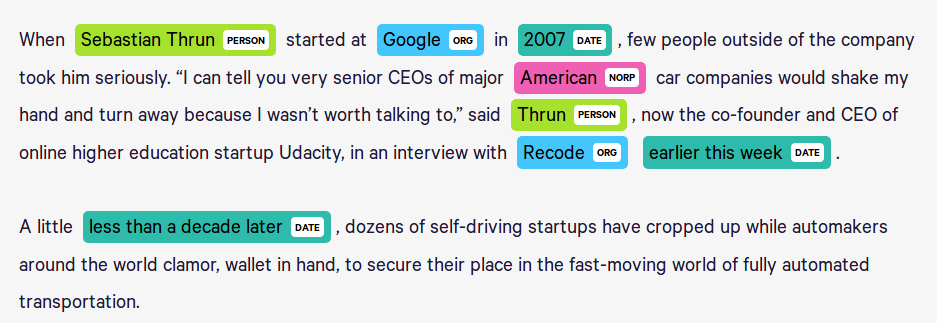
\includegraphics[width=\linewidth,keepaspectratio]{ner11}
\end{center}


	{\tiny (Ref: Complete Tutorial on Named Entity Recognition (NER) using Python and Keras - Akshay Chavan)}
\end{frame}




%%%%%%%%%%%%%%%%%%%%%%%%%%%%%%%%%%%%%%%%%%%%%%%%%%%%%%%%%%%%%%%%%%%%%%%%%%%%%%%%%%
\begin{frame}[fragile]\frametitle{The who, where, when \& how much in a sentence}
The task: identify atomic elements of information in text
  \begin{itemize}
  \item Person names
  \item Company/organization names
  \item Locations
  \item Dates \& times
  \item Percentages
  \item Monetary amounts
  \end{itemize}
  \begin{center}
\includegraphics[width=0.8\linewidth,keepaspectratio]{ner2}
\end{center}
\end{frame}


%%%%%%%%%%%%%%%%%%%%%%%%%%%%%%%%%%%%%%%%%%%%%%%%%%%%%%%%%%%%%%%%%%%%%%%%%%%%%%%%%%
\begin{frame}[fragile]\frametitle{Example}

  \begin{center}
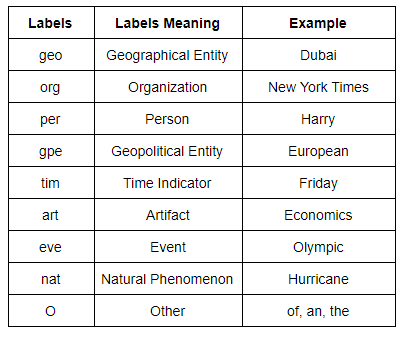
\includegraphics[width=0.6\linewidth,keepaspectratio]{ner12}
\end{center}


	{\tiny (Ref: Complete Tutorial on Named Entity Recognition (NER) using Python and Keras - Akshay Chavan)}
\end{frame}



%%%%%%%%%%%%%%%%%%%%%%%%%%%%%%%%%%%%%%%%%%%%%%%%%%%%%%%%%%%%%%%%%%%%%%%%%%%%%%%%%%
\begin{frame}[fragile]\frametitle{Difficulties}
  \begin{itemize}
  \item Too numerous to include in dictionaries
  \item Changing constantly: new names invent unknown words
  \item Appear in many variant forms: e.g. John Smith, Mr Smith, John
  \item Subsequent occurrences might be abbreviated
  \item List search/matching does't perform well
  \end{itemize}
\end{frame}

%%%%%%%%%%%%%%%%%%%%%%%%%%%%%%%%%%%%%%%%%%%%%%%%%%%%%%%%%%%%%%%%%%%%%%%%%%%%%%%%%%
\begin{frame}[fragile]\frametitle{Concept}
Whether a phrase is a proper name, and what name class it has, depends on

  \begin{itemize}
  \item Internal structure:``Mr. London'' 
  \item Context:``The new location, London, will make a better place.''
  \end{itemize}
\end{frame}

%%%%%%%%%%%%%%%%%%%%%%%%%%%%%%%%%%%%%%%%%%%%%%%%%%%%%%%%%%%%%%%%%%%%%%%%%%%%%%%%%%
\begin{frame}[fragile]\frametitle{Applications}
  \begin{itemize}
  \item Information Extraction:  relations are associations between named entities
  \item Named entities can be indexed, linked off, etc.
  \item Sentiment can be attributed to companies or products
  \item Summary generation
  \item Machine Translation
  \item Document organization/classification
  \item Increase accuracy of Internet search results (location Clinton/South Carolina vs. President Clinton)
  \item For question answering, answers are often named entities
  \end{itemize}
\end{frame}

%%%%%%%%%%%%%%%%%%%%%%%%%%%%%%%%%%%%%%%%%%%%%%%%%%%%%%%%%%%%%%%%%%%%%%%%%%%%%%%%%%
\begin{frame}[fragile]\frametitle{Standard Approaches}
  \begin{itemize}
  \item Hand-written regular expressions:  Perhaps stacked
  \item Using classifiers: Naïve Bayes, Maxent models
  \item Sequence models:HMMs, CRFs
  \end{itemize}
\end{frame}

%%%%%%%%%%%%%%%%%%%%%%%%%%%%%%%%%%%%%%%%%%%%%%%%%%%%%%%%%%%%%%%%%%%%%%%%%%%%%%%%%%
\begin{frame}[fragile]\frametitle{The hand-crafted/Rule-based approach}
Uses hand-written context-sensitive reduction rules:
  \begin{itemize}
  \item For certain restricted, common types of entities in unstructured 
text, simple regex patterns also usually work.
  \item Finding (US) phone numbers
  \item \lstinline| (?:\(?[0-9]{3}\)?[ -.])?[0-9]{3}[ -.]?[0-9]{4}|
  \item Title capitalized word : title person\_name compare ``Mr. Jones'' vs. ``Mr. Ten-Percent'' : no rule without exceptions
  \item  person\_name, ``the'' adj* ``CEO of'' organization ``Fred Smith, the young dynamic CEO of BlubbCo'' : ability to grasp non-local patterns
  \end{itemize}
  Plus help from databases of known named entities

\end{frame}

%%%%%%%%%%%%%%%%%%%%%%%%%%%%%%%%%%%%%%%%%%%%%%%%%%%%%%%%%%%%%%%%%%%%%%%%%%%%%%%%%%
\begin{frame}[fragile]\frametitle{Word Features}
Easily determinable token properties:
\begin{center}
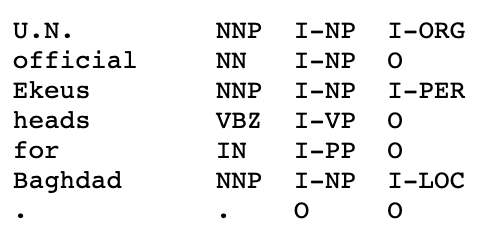
\includegraphics[width=\linewidth,keepaspectratio]{ner1}
\end{center}
\end{frame}

%%%%%%%%%%%%%%%%%%%%%%%%%%%%%%%%%%%%%%%%%%%%%%%%%%%%%%%%%%%%%%%%%%%%%%%%%%%%%%%%%%
\begin{frame}[fragile]\frametitle{MUC: the NLP genesis of IE}
  \begin{itemize}
  \item DARPA funded significant efforts in IE in the early to mid 1990s
  \item Message Understanding Conference (MUC) was an annual event/competition where results were presented.
  \item Focused on extracting information from news articles: Terrorist events, Industrial joint ventures, Company management changes
  \item Starting off, all rule-based, gradually moved to ML
  \end{itemize}
\end{frame}

%%%%%%%%%%%%%%%%%%%%%%%%%%%%%%%%%%%%%%%%%%%%%%%%%%%%%%%%%%%%%%%%%%%%%%%%%%%%%%%%%%
\begin{frame}[fragile]\frametitle{Example from MUC-7}
Delimit the named entities in a text and tag them with NE categores:

  \begin{lstlisting}
<ENAMEX TYPE=``LOCATION''>Italy</ENAMEX>'s business world was rocked by
the announcement <TIMEX TYPE=``DATE''>last Thursday</TIMEX> that Mr.
<ENAMEX TYPE=``PERSON''>Verdi</ENAMEX> would leave his job as vice-president
of <ENAMEX TYPE=``ORGANIZATION''>Music Masters of Milan, Inc</ENAMEX> 
to become operations director of  
<ENAMEX TYPE=``ORGANIZATION''>Arthur Andersen</ENAMEX>.
  \end{lstlisting}
  
  \begin{itemize}
  \item ``Milan'' is part of organization name
  \item ``Arthur Andersen'' is a company 
  \item ``Italy'' is sentence-initial : capitalization useless
  \end{itemize}
\end{frame}

%%%%%%%%%%%%%%%%%%%%%%%%%%%%%%%%%%%%%%%%%%%%%%%%%%%%%%%%%%%%%%%%%%%%%%%%%%%%%%%%%%
\begin{frame}[fragile]\frametitle{Hand-written Information Extraction}
For unstructured human-written text, some NLP may help
  \begin{itemize}
  \item Part-of-speech (POS) tagging: Mark each word as a noun, verb, preposition, etc.
  \item Syntactic parsing: Identify phrases: NP, VP, PP
  \item Semantic word categories (e.g. from WordNet): KILL: kill, murder, assassinate, strangle, suffocate
  \end{itemize}
\end{frame}





%%%%%%%%%%%%%%%%%%%%%%%%%%%%%%%%%%%%%%%%%%%%%%%%%%%%%%%%%%%%%%%%%%%%%%%%%%%%%%%%%%
\begin{frame}[fragile]\frametitle{The Automated ML sequence model approach to NER}
Training
  \begin{itemize}
  \item  Collect a set of representative training documents
  \item  Label each token for its entity class or other (O)
  \item  Design feature extractors appropriate to the text and classes 3. Design feature extractors appropriate to the text and classes
  \item  Train a sequence classifier to predict the labels from the data
  \end{itemize}
Testing  
  \begin{itemize}
  \item  Receive a set of testing documents
  \item  Run sequence model inference to label each token
  \item  Appropriately output the recognized entities
  \end{itemize}
\end{frame}

%%%%%%%%%%%%%%%%%%%%%%%%%%%%%%%%%%%%%%%%%%%%%%%%%%%%%%%%%%%%%%%%%%%%%%%%%%%%%%%%%%
\begin{frame}[fragile]\frametitle{Terminology}
  \begin{itemize}
  \item History $h_t$: information derivable from the corpus relative to a token $t$:
    \begin{itemize}
  \item text window around token $w-i$, e.g. $w_{i-2},\ldots,w_{i+2}$
  \item word features of these tokens
  \item POS, other complex features
    \end{itemize}
  \item Binary features: yes/no-questions on history used by models to determine probabilities of
  \item Futures: name classes

  \end{itemize}
\end{frame}

%%%%%%%%%%%%%%%%%%%%%%%%%%%%%%%%%%%%%%%%%%%%%%%%%%%%%%%%%%%%%%%%%%%%%%%%%%%%%%%%%%
\begin{frame}[fragile]\frametitle{Encoding classes for sequence labeling}

\begin{center}
\includegraphics[width=0.8\linewidth,keepaspectratio]{ner3}

\includegraphics[width=\linewidth,keepaspectratio]{ner5}
\end{center}
\end{frame}

%%%%%%%%%%%%%%%%%%%%%%%%%%%%%%%%%%%%%%%%%%%%%%%%%%%%%%%%%%%%%%%%%%%%%%%%%%%%%%%%%%
\begin{frame}[fragile]\frametitle{CoNLL-2003}
  \begin{itemize}
  \item CoNLL - Conference on Natural Language Learning by the ACL's Special Interest Group on Natural Language Learning
  \item Shared Task: Language-Independent Named Entity Recognition
  \item Goal: Identify boundaries and types of named entities
\begin{center}
\includegraphics[width=0.5\linewidth,keepaspectratio]{ner9}
\end{center}
\item Inputs: $x = (x_1,\ldots, x_n)$
\item Labels: $y = (y_1,\ldots, y_n)$
\item Typical goal: Given $x$, predict $y$

  \end{itemize}
\end{frame}

%%%%%%%%%%%%%%%%%%%%%%%%%%%%%%%%%%%%%%%%%%%%%%%%%%%%%%%%%%%%%%%%%%%%%%%%%%%%%%%%%%
\begin{frame}[fragile]\frametitle{Methods for Sequence Labeling}
Typically the following methods are used for NER:
  \begin{itemize}
  \item Hidden Markov Model (HMM)
  \item Maximum Entropy Classifier (MaxEnt)
  \item Maximum Entropy Markov Model (MEMM)
  \item Conditional Random Fields (CRF)
  \end{itemize}
These are all classifiers (i.e., supervised learning) which model sequences (rather than individual random variables)
\end{frame}


%%%%%%%%%%%%%%%%%%%%%%%%%%%%%%%%%%%%%%%%%%%%%%%%%%%%%%%%%%%%%%%%%%%%%%%%%%%%%%%%%%
\begin{frame}[fragile]\frametitle{Features for sequence labeling}
  \begin{itemize}
  \item Words:
  \begin{itemize}
  \item Current word (essentially like a learned dictionary)
  \item Previous/next word (context)
  \end{itemize}
  \item Other kinds of inferred linguistic classification: Part-of-speech tags
  \item Label context: Previous (and perhaps next) label
  \item Word Shapes: Map words to simplified representation that encodes attributes such as length, capitalization, numerals, Greek letters, internal punctuation, etc.
\begin{center}
\includegraphics[width=0.4\linewidth,keepaspectratio]{ner4}
\end{center}
  \end{itemize}
\end{frame}

%%%%%%%%%%%%%%%%%%%%%%%%%%%%%%%%%%%%%%%%%%%%%%%%%%%%%%%%%%%%%%%%%%%%%%%%%%%%%%%%%%
\begin{frame}[fragile]\frametitle{Maximum Entropy Markov Model (MEMM)}
  \begin{itemize}
  \item (MEMM) classifier makes a single decision at a time, conditioned on evidence from observations and previous decisions.
  \item Scoring individual labeling decisions is no more complex than standard classification decisions. Using features for classification.
  \end{itemize}
\begin{center}
\includegraphics[width=\linewidth,keepaspectratio]{ner6}
\end{center}
\end{frame}

%%%%%%%%%%%%%%%%%%%%%%%%%%%%%%%%%%%%%%%%%%%%%%%%%%%%%%%%%%%%%%%%%%%%%%%%%%%%%%%%%%
\begin{frame}[fragile]\frametitle{Hidden Markov Models (HMMs)}
\begin{center}
\includegraphics[width=\linewidth,keepaspectratio]{ner10}
\end{center}
\end{frame}

%%%%%%%%%%%%%%%%%%%%%%%%%%%%%%%%%%%%%%%%%%%%%%%%%%%%%%%%%%%%%%%%%%%%%%%%%%%%%%%%%%
\begin{frame}[fragile]\frametitle{Viterbi Inference}
  \begin{itemize}
  \item Dynamic programming or memoization.
  \item Requires small window of state influence (e.g., past two states are relevant).
  \item Advantage:: Exact: the global best sequence is returned.
  \item Disadvantage: Harder to implement long-distance state-state interactions (but beam inference tends not
to allow long-distance resurrection of sequences anyway).
  \end{itemize}
\begin{center}
\includegraphics[width=\linewidth,keepaspectratio]{ner7}
\end{center}
\end{frame}

%%%%%%%%%%%%%%%%%%%%%%%%%%%%%%%%%%%%%%%%%%%%%%%%%%%%%%%%%%%%%%%%%%%%%%%%%%%%%%%%%%
\begin{frame}[fragile]\frametitle{Viterbi Inference}
\begin{center}
\includegraphics[width=\linewidth,keepaspectratio]{ner8}
\end{center}
\end{frame}

%%%%%%%%%%%%%%%%%%%%%%%%%%%%%%%%%%%%%%%%%%%%%%%%%%%%%%%%%%%%%%%%%%%%%%%%%%%%%%%%%%
\begin{frame}[fragile]\frametitle{Viterbi Inference}
  \begin{itemize}
  \item Create an array, with columns corresponding to inputs, rows corresponding to possible states
  \item Sweep through the array in one pass filling the columns left to right using our transition probs and observations probs
  \item Dynamic programming key is that we need only store the MAX prob path to each cell, (not all paths).
  \end{itemize}
\end{frame}

%%%%%%%%%%%%%%%%%%%%%%%%%%%%%%%%%%%%%%%%%%%%%%%%%%%%%%%%%%%%%%%%%%%%%%%%%%%%%%%%%%
\begin{frame}[fragile]\frametitle{Conditional Random Fields (CRFs)}
  \begin{itemize}
  \item CRFs are used for predicting the sequences that use the contextual information to add information which will be used by the model to make a correct prediction.
	\item The output sequence is modeled as the normalized product of the feature function.
  \end{itemize}
	
	\begin{center}
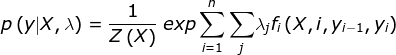
\includegraphics[width=0.5\linewidth,keepaspectratio]{ner13}
\end{center}
\end{frame}


%%%%%%%%%%%%%%%%%%%%%%%%%%%%%%%%%%%%%%%%%%%%%%%%%%%%%%%%%%%%%%%%%%%%%%%%%%%%%%%%%%
\begin{frame}[fragile]\frametitle{Feature Preparation for CRF}

\begin{center}
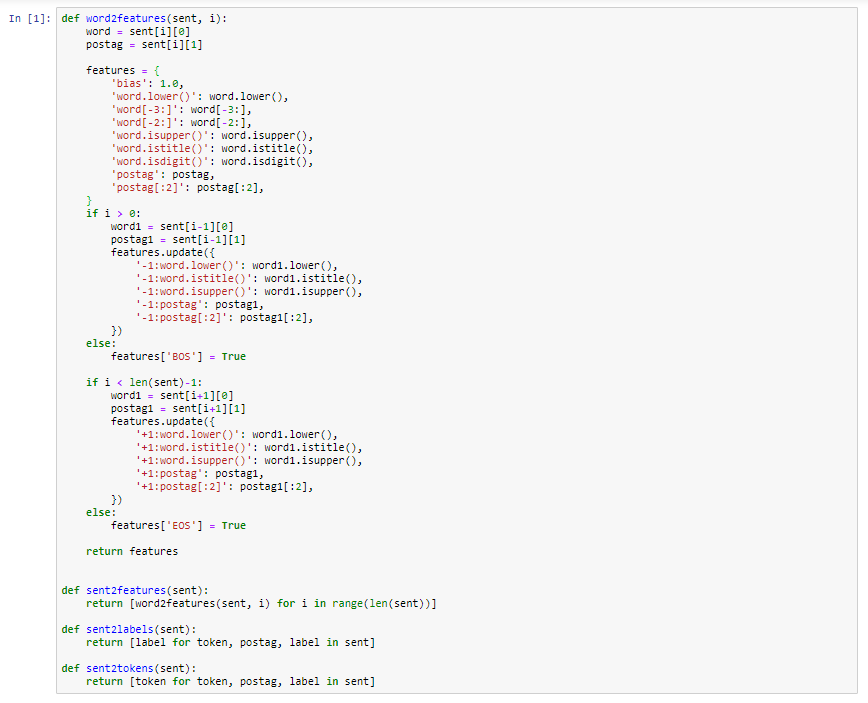
\includegraphics[width=0.8\linewidth,keepaspectratio]{ner14}
\end{center}

\end{frame}

%%%%%%%%%%%%%%%%%%%%%%%%%%%%%%%%%%%%%%%%%%%%%%%%%%%%%%%%%%%%%%%%%%%%%%%%%%%%%%%%%%
\begin{frame}[fragile]\frametitle{Training the model with scikit-learn}

\begin{center}
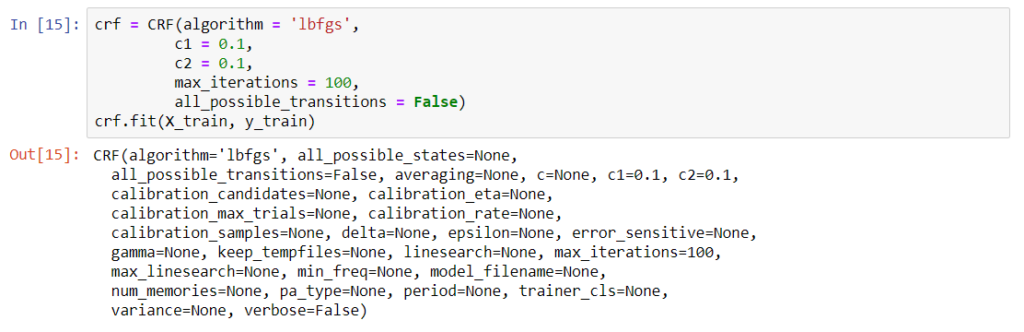
\includegraphics[width=\linewidth,keepaspectratio]{ner15}
\end{center}

\end{frame}

%%%%%%%%%%%%%%%%%%%%%%%%%%%%%%%%%%%%%%%%%%%%%%%%%%%%%%%%%%%%%%%%%%%%%%%%%%%%%%%%%%
\begin{frame}[fragile]\frametitle{Evaluating the model  performance}

\begin{center}
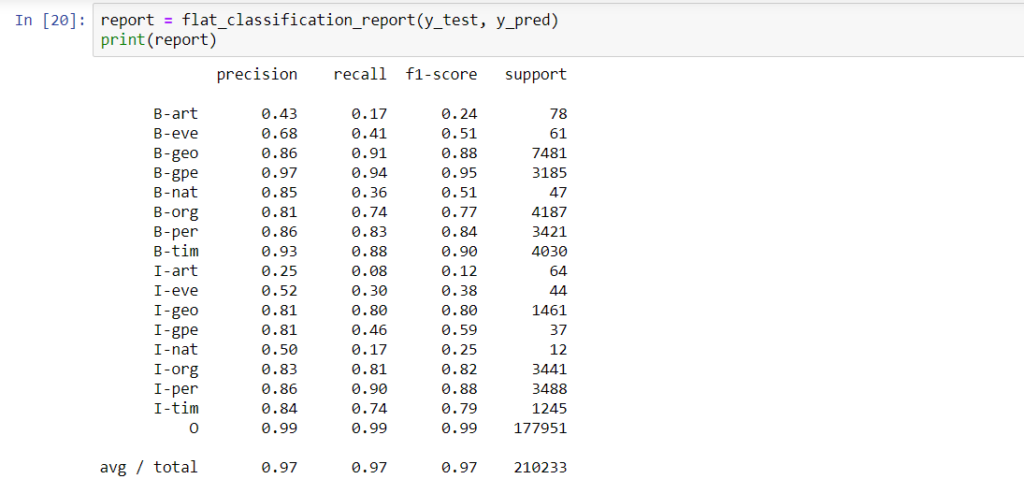
\includegraphics[width=\linewidth,keepaspectratio]{ner16}
\end{center}

\end{frame}

%%%%%%%%%%%%%%%%%%%%%%%%%%%%%%%%%%%%%%%%%%%%%%%%%%%%%%%%%%%%%%%%%%%%%%%%%%%%%%%%%%
\begin{frame}[fragile]\frametitle{Hand-crafted vs. Automated }
Hand-made systems:
  \begin{itemize}
  \item Can achieve higher performance than ML systems
  \item Non-local phenomena best handled by regular expressions
  \item Several person-months for rule-writing, requires experienced linguists
  \item Rules depend on specific properties of language, domain \& text format  
  \item Manual adaption necessary when domain changes
  \item Re-write rules for other languages
  \end{itemize}
\end{frame}

%%%%%%%%%%%%%%%%%%%%%%%%%%%%%%%%%%%%%%%%%%%%%%%%%%%%%%%%%%%%%%%%%%%%%%%%%%%%%%%%%%
\begin{frame}[fragile]\frametitle{Hand-crafted vs. Automated }
Automated approaches:
  \begin{itemize}
  \item Train on human-annotated texts
  \item No expensive computational linguists needed
  \item 1,00,000 words can be tagged in 1-3 days
  \item Ideally, no manual work required for domain changes
  \item Easier to port to other languages
  \item Features are locally limited
  \end{itemize}
\end{frame}

%%%%%%%%%%%%%%%%%%%%%%%%%%%%%%%%%%%%%%%%%%%%%%%%%%%%%%%%%%%%%%%%%%%%%%%%%%%%%%%%%%
\begin{frame}[fragile]\frametitle{Evaluation for NER }
  \begin{itemize}
  \item Recall and precision are straightforward for tasks like IR and text 
categorization, where there is only one grain size (documents)
  \item The measure behaves a bit funnily for IE/NER when there are 
boundary errors (which are common):
  \item First Bank of Chicago announced earnings
  \item This counts as both a FP and a FN
  \item Selecting nothing would have been better
  \item Some other metrics (e.g., MUC scorer) give partial credit (according to complex rules)
  \end{itemize}
\end{frame}



%%%%%%%%%%%%%%%%%%%%%%%%%%%%%%%%%%%%%%%%%%%%%%%%%%%%%%%%%%%%%%%%%%%%%%%%%%%%%%%%%
\begin{frame}[fragile]\frametitle{}

\begin{center}
{\Large NER with NLTK}
\end{center}
\end{frame}

%%%%%%%%%%%%%%%%%%%%%%%%%%%%%%%%%%%%%%%%%%%%%%%%%%%%%%%%%%%%%%%%%%%%%%%%%%%%%%%%%%
\begin{frame}[fragile]\frametitle{Steps for NER}
  \begin{itemize}
  \item Take a string as input
  \item Tokenize it into sentences
  \item Tokenize the sentences into words
  \item Add part-of-speech tags to the words using \lstinline|nltk.pos_tag()|
  \item  Run this through the NLTK-provided NER classifier using \lstinline|nltk.ne_chunk()|
  \item  Parse these intermediate results and return any extracted entities

  \end{itemize}
\end{frame}


%%%%%%%%%%%%%%%%%%%%%%%%%%%%%%%%%%%%%%%%%%%%%%%%%%%%%%%%%%%%%%%%%%%%%%%%%%%%%%%%%%
\begin{frame}[fragile]\frametitle{NLTK NER Chunker}
  \begin{itemize}
  \item \lstinline|ne_chunk| needs part-of-speech annotations to add NE labels to the sentence. The output of the \lstinline|ne_chunk| is a \lstinline|nltk.Tree| object.
  \begin{lstlisting}
from nltk import word_tokenize, pos_tag, ne_chunk
sentence = "Mark and John are working at Google."
print ne_chunk(pos_tag(word_tokenize(sentence)))
"""
(S
  (PERSON Mark/NNP)
  and/CC
  (PERSON John/NNP)
  are/VBP
  working/VBG
  at/IN
  (ORGANIZATION Google/NNP)
  ./.)
"""
  \end{lstlisting}
  \end{itemize}
\end{frame}


%%%%%%%%%%%%%%%%%%%%%%%%%%%%%%%%%%%%%%%%%%%%%%%%%%%%%%%%%%%%%%%%%%%%%%%%%%%%%%%%%%
\begin{frame}[fragile]\frametitle{Steps for NER}
  \begin{itemize}
  \item NLTK provides a classifier that has already been trained to recognize named entities, accessed with the function \lstinline|nltk.ne_chunk()|. 
\item If we set the parameter \lstinline|binary=True|, then named entities are just tagged as \lstinline|NE|; otherwise, the classifier adds category labels such as \lstinline|PERSON, ORGANIZATION, and GPE|.
  \begin{lstlisting}
 >>> print(nltk.ne_chunk(sent)) 
(S
  The/DT
  (GPE U.S./NNP)
  is/VBZ
  one/CD
  ...
  according/VBG
  to/TO
  (PERSON Brooke/NNP T./NNP Mossman/NNP)
  ...)
  \end{lstlisting}
  \end{itemize}
\end{frame}

%%%%%%%%%%%%%%%%%%%%%%%%%%%%%%%%%%%%%%%%%%%%%%%%%%%%%%%%%%%%%%%%%%%%%%%%%%%%%%%%%%
\begin{frame}[fragile]\frametitle{IOB tagging}
The IOB Tagging system contains tags of the form:
  \begin{itemize}
  \item \lstinline|B-{CHUNK_TYPE}| - for the word in the Beginning chunk
  \item \lstinline|I-{CHUNK_TYPE}| - for words Inside the chunk
  \item \lstinline|O| - Outside any chunk
  \end{itemize}

\end{frame}

%%%%%%%%%%%%%%%%%%%%%%%%%%%%%%%%%%%%%%%%%%%%%%%%%%%%%%%%%%%%%%%%%%%%%%%%%%%%%%%%%%
\begin{frame}[fragile]\frametitle{IOB tagging}
  \begin{lstlisting}
from nltk.chunk import conlltags2tree, tree2conlltags
sentence = "Mark and John are working at Google."
ne_tree = ne_chunk(pos_tag(word_tokenize(sentence)))
iob_tagged = tree2conlltags(ne_tree)
print iob_tagged
"""[('Mark', 'NNP', u'B-PERSON'), ('and', 'CC', u'O'), ('John', 'NNP', u'B-PERSON'), ('are', 'VBP', u'O'), ('working', 'VBG', u'O'), ('at', 'IN', u'O'), ('Google', 'NNP', u'B-ORGANIZATION'), ('.', '.', u'O')]
"""
ne_tree = conlltags2tree(iob_tagged)
print ne_tree
""" (S
  (PERSON Mark/NNP)
  and/CC
  (PERSON John/NNP)
  are/VBP
  working/VBG
  at/IN
  (ORGANIZATION Google/NNP)
  ./.)
"""
\end{lstlisting}
\end{frame}

%%%%%%%%%%%%%%%%%%%%%%%%%%%%%%%%%%%%%%%%%%%%%%%%%%%%%%%%%%%%%%%%%%%%%%%%%%%%%%%%%%%
%\begin{frame}[fragile]\frametitle{Max Entropy}
%  \begin{lstlisting}
%import nltk
%nltk.download('maxent_ne_chunker')
%nltk.download('words')
%import re
%import time
%contentArray =['Starbucks is not doing very well lately.',
%               'Overall, while it may seem there is already a Starbucks on every corner, Starbucks still has a lot of room to grow.',
%               'Increase in supply... well you know the rules...',]
%for item in contentArray:
%            tokenized = nltk.word_tokenize(item)
%            tagged = nltk.pos_tag(tokenized)
%            #print tagged
%             namedEnt = nltk.ne_chunk(tagged)
%            namedEnt.draw()
%  \end{lstlisting}
%\end{frame}

%%%%%%%%%%%%%%%%%%%%%%%%%%%%%%%%%%%%%%%%%%%%%%%%%%%%%%%%%%%%%%%%%%%%%%%%%%%%%%%%%%
\begin{frame}[fragile]\frametitle{NLTK.Stanford NER}
  \begin{lstlisting}
wget "http://nlp.stanford.edu/software/stanford-ner-2014-06-16.zip"
unzip stanford-ner-2014-06-16.zip
mv stanford-ner-2014-06-16 stanford-ner
sudo mv stanford-ner /usr/share/

from nltk import word_tokenize
from nltk.tag.stanford import NERTagger
 
classifier = '/usr/share/stanford-ner/classifiers/english.all.3class.distsim.crf.ser.gz'
jar = '/usr/share/stanford-ner/stanford-ner.jar'
st = NERTagger(classifier,jar)
sentence = word_tokenize("Rami Eid is studying at Stony Brook University in NY")
print st.tag(sentence)
  \end{lstlisting}
\end{frame}
%%%%%%%%%%%%%%%%%%%%%%%%%%%%%%%%%%%%%%%%%%%%%%%%%%%%%%%%%%%%%%%%%%%%%%%%%%%%%%%%%%
\begin{frame}[fragile]\frametitle{}

\begin{center}
{\Large NER with Spacy}
\end{center}
\end{frame}


%%%%%%%%%%%%%%%%%%%%%%%%%%%%%%%%%%%%%%%%%%%%%%%%%%%%%%%%%%%%%%%%%%%%%%%%%%%%%%%%%%
\begin{frame}[fragile]\frametitle{Spacy}
  \begin{itemize}
  \item SpaCy is an open-source python library for NLP written in Python and Cython. 
	\item Offers pre-trained models for multi-language NER, as well as allowing developers to train and deploy custom NER models on domain specific corpuses. 
	\item SpaCy models are designed to be production-ready.
	\item Uses 1D residual convolutional neural networks (CNN) and incremental parsing with Bloom embeddings for NER
  \end{itemize}
	
	{\tiny (Ref: Google Cloud AI Hub Named Entity Recognition using Spacy and Tensorflow)}
\end{frame}

%%%%%%%%%%%%%%%%%%%%%%%%%%%%%%%%%%%%%%%%%%%%%%%%%%%%%%%%%%%%%%%%%%%%%%%%%%%%%%%%%%
\begin{frame}[fragile]\frametitle{Spacy Default NER}
Identifies:
  \begin{itemize}
  \item PERSON:	People, including fictional
	\item ORG:	Companies, agencies, institutions, etc
	\item GPE:	Countries, cities, states
	\item PRODUCT:	Objects, vehicles, foods, etc. (Not services.)
	\item DATE:	Absolute or relative dates or periods
	\item TIME:	Times smaller than a day
	\item PERCENT:	Percentage, including ”%“
	\item MONEY:	Monetary values, including unit
	\item QUANTITY:	Measurements, as of weight or distance
	\item \ldots
  \end{itemize}
	
	{\tiny (Ref: Google Cloud AI Hub Named Entity Recognition using Spacy and Tensorflow)}
\end{frame}

%%%%%%%%%%%%%%%%%%%%%%%%%%%%%%%%%%%%%%%%%%%%%%%%%%%%%%%%%%%%%%%%%%%%%%%%%%%%%%%%%%
\begin{frame}[fragile]\frametitle{Spacy Default NER}

\begin{lstlisting}
import spacy
nlp = spacy.load('en_core_web_sm')

doc = nlp("Indians spent over $71 billion on clothes in 2018")
 
for ent in doc.ents:
    print(ent.text, ent.label_)
		
Indians NORP
over $71 billion MONEY
2018 DATE

spacy.explain("NORP")
Output: `Nationalities religious or political groups'
\end{lstlisting}
	
	{\tiny (Ref: spaCy Tutorial to Learn and Master Natural Language Processing (NLP) - Prateek Joshi - Analytics Vidhya)}
\end{frame}


%%%%%%%%%%%%%%%%%%%%%%%%%%%%%%%%%%%%%%%%%%%%%%%%%%%%%%%%%%%%%%%%%%%%%%%%%%%%%%%%%%
\begin{frame}[fragile]\frametitle{Named Entity Recognition NER}

\begin{lstlisting}
text = 'Apple is looking for buying a U.K. startup. Government has given permission.'

doc = nlp(text)
print(doc)

>> Apple is looking for buying a U.K. startup for $1 billion

for token in doc:
    print(token.text, token.label_)

Apple ORG
U.K. GPE
$1 billion MONEY

doc = nlp('Apple is looking for buying a UK startup for $1 billion in 2020')
displacy.render(doc, style = 'ent')
\end{lstlisting}

\begin{center}

\includegraphics[width=0.8\linewidth,keepaspectratio]{spacy6}
\end{center}

{\tiny (Ref: https://spacy.io/usage/spacy-101)}
\end{frame}


%%%%%%%%%%%%%%%%%%%%%%%%%%%%%%%%%%%%%%%%%%%%%%%%%%%%%%%%%%%%%%%%%%%%%%%%%%%%%%%%%%
\begin{frame}[fragile]\frametitle{}

\begin{center}
{\Large Custom NER}
\end{center}
\end{frame}

%%%%%%%%%%%%%%%%%%%%%%%%%%%%%%%%%%%%%%%%%%%%%%%%%%%%%%%%%%%%%%%%%%%%%%%%%%%%%%%%%%
\begin{frame}[fragile]\frametitle{Training your own NER}
  \begin{itemize}
  \item Either rule-based or machine learning (ML) based.
	\item Requires a large amount of labeled training data
	\item ML approaches from scratch: Hidden Markov Models, Maximum Entropy, and Conditional Random Fields, as well as deep learning approaches with Recurrent Neural Networks, such as Seq2Seq
	\item Need sentence inputs and annotated sentence outputs. 
	\item May also involve additional feature engineering
	\item Some libraries like Spacy and Stanford allow training of custom NER.
  \end{itemize}
\end{frame}


%%%%%%%%%%%%%%%%%%%%%%%%%%%%%%%%%%%%%%%%%%%%%%%%%%%%%%%%%%%%%%%%%%%%%%%%%%%%%%%%%%
\begin{frame}[fragile]\frametitle{NER Datasets}
  \begin{itemize}
  \item Domain-specific (i.e. Twitter, biomedical, advertising, news).
	\item i2b2 - Medication, treatments, diseases, risk factors, and medications
	\item CoNLL 2003 - English and german news articles annotated with location, organization, person, and miscellaneous
  \end{itemize}
\end{frame}


%%%%%%%%%%%%%%%%%%%%%%%%%%%%%%%%%%%%%%%%%%%%%%%%%%%%%%%%%%%%%%%%%%%%%%%%%%%%%%%%%%
\begin{frame}[fragile]\frametitle{NER Evaluation metrics}
  \begin{itemize}
  \item NER is most commonly evaluated with precision, recall, and F1-score.
  \end{itemize}
\end{frame}


%%%%%%%%%%%%%%%%%%%%%%%%%%%%%%%%%%%%%%%%%%%%%%%%%%%%%%%%%%%%%%%%%%%%%%%%%%%%%%%%%%
\begin{frame}[fragile]\frametitle{Training your own system}
  \begin{itemize}
  \item The feature extraction works almost identical as the one implemented in the Training a Part-Of-Speech Tagger, except need to add many features.
  \item Since the previous IOB tag is a very good indicator of what the current IOB tag is going to be, we have included the previous IOB tag as a feature.
  \item Spacy Provides Gold Parse method
  \item CRF++ can be used to generate custom NER tags.
  \end{itemize}
\end{frame}

%%%%%%%%%%%%%%%%%%%%%%%%%%%%%%%%%%%%%%%%%%%%%%%%%%%%%%%%%%%%%%%%%%%%%%%%%%%%%%%%%%
\begin{frame}[fragile]\frametitle{}

\begin{center}
{\Large Spacy Custom NER}
\end{center}
\end{frame}

%%%%%%%%%%%%%%%%%%%%%%%%%%%%%%%%%%%%%%%%%%%%%%%%%%%%%%%%%%
\begin{frame}[fragile]\frametitle{Custom NER Process}


\begin{center}
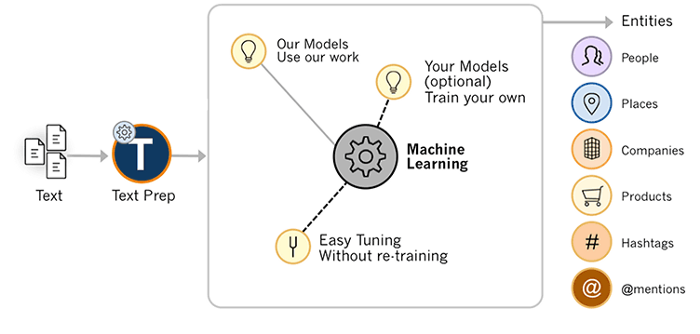
\includegraphics[width=0.8\linewidth,keepaspectratio]{ie15}
\end{center}

{\tiny (Ref: Training Custom NER - Nishanth N)}

\end{frame}

%%%%%%%%%%%%%%%%%%%%%%%%%%%%%%%%%%%%%%%%%%%%%%%%%%%%%%%%%%
\begin{frame}[fragile]\frametitle{Training Data Format}


\begin{lstlisting}

TRAIN_DATA = [
    ('Who is Nishanth?', {
        'entities': [(7, 15, 'PERSON')]
    }),
     ('Who is Kamal Khumar?', {
        'entities': [(7, 19, 'PERSON')]
    }),
    ('I like London and Berlin.', {
        'entities': [(7, 13, 'LOC'), (18, 24, 'LOC')]
    })
]
\end{lstlisting}

{\tiny (Ref: Training Custom NER - Nishanth N)}

\end{frame}

%%%%%%%%%%%%%%%%%%%%%%%%%%%%%%%%%%%%%%%%%%%%%%%%%%%%%%%%%%
\begin{frame}[fragile]\frametitle{NER Pipeline}


\begin{lstlisting}

nlp = spacy.load(model)  
ner = nlp.create_pipe('ner')
nlp.add_pipe(ner, last=True)

for _, annotations in TRAIN_DATA:
    for ent in annotations.get('entities'):
        ner.add_label(ent[2])
				
# Disable pipeline components you dont need to change
pipe_exceptions = ["ner", "trf_wordpiecer", "trf_tok2vec"]
unaffected_pipes = [pipe for pipe in nlp.pipe_names if pipe not in pipe_exceptions]

\end{lstlisting}

{\tiny (Ref: Training Custom NER - Nishanth N)}

\end{frame}

%%%%%%%%%%%%%%%%%%%%%%%%%%%%%%%%%%%%%%%%%%%%%%%%%%%%%%%%%%
\begin{frame}[fragile]\frametitle{Training}


\begin{lstlisting}
# Disable pipeline components you dont need to change
other_pipes = [pipe for pipe in nlp.pipe_names if pipe != 'ner']
with nlp.disable_pipes(*other_pipes):  # only train NER
    optimizer = nlp.begin_training()
    for itn in range(n_iter):
        random.shuffle(TRAIN_DATA)
        losses = {}
        for text, annotations in tqdm(TRAIN_DATA):
            nlp.update(
                [text],  
                [annotations],  
                drop=0.5,  
                sgd=optimizer,
                losses=losses)
        print(losses)
\end{lstlisting}

{\tiny (Ref: Training Custom NER - Nishanth N)}

\end{frame}

%%%%%%%%%%%%%%%%%%%%%%%%%%%%%%%%%%%%%%%%%%%%%%%%%%%%%%%%%%
\begin{frame}[fragile]\frametitle{Testing}


\begin{lstlisting}
doc = nlp("I was driving a Alto")
print("Entities", [(ent.text, ent.label_) for ent in doc.ents])
\end{lstlisting}

{\tiny (Ref: Training Custom NER - Nishanth N)}

\end{frame}

\section[Topics]{Topic Modeling}
%%%%%%%%%%%%%%%%%%%%%%%%%%%%%%%%%%%%%%%%%%%%%%%%%%%%%%%%%%%%%%%%%%%%%%%%%%%%%%%%%%
\begin{frame}[fragile]\frametitle{}

\begin{center}
{\Large Topic Modeling}
\end{center}
\end{frame}

%%%%%%%%%%%%%%%%%%%%%%%%%%%%%%%%%%%%%%%%%%%%%%%%%%%%%%%%%%%%%%%%%%%%%%%%%%%%%%%%%%
\begin{frame}[fragile]\frametitle{What is Topic Modeling?}
  \begin{itemize}
  	\item Topic modeling is a form of text mining, a way of identifying patterns in a corpus. 
	\item  You take your corpus and run it through a tool which groups words across the corpus into `topics' ( clusters of words) by a process of similarity.
	\item In a good topic model, the words in topic make sense, for example ``navy, ship, captain'' and ``tobacco, farm, crops.''
  \end{itemize}
\begin{center}
\includegraphics[width=0.6\linewidth,keepaspectratio]{top}
\end{center}
\end{frame}

%%%%%%%%%%%%%%%%%%%%%%%%%%%%%%%%%%%%%%%%%%%%%%%%%%%%%%%%%%%%%%%%%%%%%%%%%%%%%%%%%%
\begin{frame}[fragile]\frametitle{Core Concept: Similarity}
Are these statements similar?
  \begin{itemize}
  	\item ``A seven-year quest to collect samples from the solar system's formation ended in triumph in a dark and wet Utah desert this weekend.''
	\item ``For a month, a huge storm with massive lightning has been raging on Jupiter under the watchful eye of an orbiting spacecraft.''
	\item ``One of Saturn's moons is spewing a giant plume of water vapour that is feeding the planet's rings, scientists say.''
  \end{itemize}
How would you quantify their similarity? How would you decide that two are more similar to each other than to the third? 

\end{frame}

%%%%%%%%%%%%%%%%%%%%%%%%%%%%%%%%%%%%%%%%%%%%%%%%%%%%%%%%%%%%%%%%%%%%%%%%%%%%%%%%%%
\begin{frame}[fragile]\frametitle{Semantic Similarity}
  \begin{itemize}
  	\item A study done in Australia in 2005 : what a sample of Australian college students think is similar. 
	\item Students read hundreds of paired short excerpts from news articles and ranked the pairwise similarity on a scale. 	
	\item Then examined all the classifications, and found that they had a correlation of 0.6. 
	\item That's obviously a positive correlation, but not terribly high. 
	\item So, humans doesn't necessarily agree with each other about semantic similarity
	\item It's kind of a fuzzy notion
  \end{itemize}
\end{frame}

%%%%%%%%%%%%%%%%%%%%%%%%%%%%%%%%%%%%%%%%%%%%%%%%%%%%%%%%%%%%%%%%%%%%%%%%%%%%%%%%%%
\begin{frame}[fragile]\frametitle{Semantic Similarity: Any number?}
  \begin{itemize}
  	\item The study mentioned found that a particular topic modelling technique called latent semantic analysis (LSA) could achieve also a 0.6 correlation with the human ratings
	\item Correlating with the study participant's choice about as well as they correlated with each other.
  \end{itemize}
\end{frame}

%%%%%%%%%%%%%%%%%%%%%%%%%%%%%%%%%%%%%%%%%%%%%%%%%%%%%%%%%%%%%%%%%%%%%%%%%%%%%%%%%%
\begin{frame}[fragile]\frametitle{Who cares about semantic similarity? }
Some use cases:

  \begin{itemize}
  	\item Query large collections of text: Traditionally used on large document collections. Legal discovery. Answer questions or aid searching huge corpora like government regulations, manuals, patent databases, etc.

  	\item  Automatic metadata: system can intelligently suggest tags and categories for documents based on other documents they're similar too. 
  	\item  Recommendations: plagiarism detection, exam scoring. And there are a number of other use cases. 
  	\item  Better human-computer interaction: Matching on similarity rather than words or with regexes allows us to accept broader ranges of input, in theory. 

  \end{itemize}
\end{frame}

%%%%%%%%%%%%%%%%%%%%%%%%%%%%%%%%%%%%%%%%%%%%%%%%%%%%%%%%%%%%%%%%%%%%%%%%%%%%%%%%%%
\begin{frame}[fragile]\frametitle{What is Topic Modeling?}
  \begin{itemize}
  	\item Topic modelling attempts to uncover the underlying semantic structure of text (or other data) by using statistical techniques to identify abstract, recurring patterns of terms in a set of data. 
  	\item These patterns are called topics. They may or may not correspond to our intuitive notion of a topic. 
	\item Topic modelling models documents as collections of features, representing the documents as long vectors that indicate the presence/absence of important features, for example, the presence or absence of words in a document. 
	\item We can use those vectors to create spaces and plot the locations of documents in those spaces and use that as a kind of proxy for their meaning.
  \end{itemize}
\end{frame}

%%%%%%%%%%%%%%%%%%%%%%%%%%%%%%%%%%%%%%%%%%%%%%%%%%%%%%%%%%%%%%%%%%%%%%%%%%%%%%%%%%
\begin{frame}[fragile]\frametitle{What is Topic Modeling?}
  \begin{itemize}
  	\item Topic modeling is an unsupervised algorithm.
  	\item One of the key ideas behind it is that every topic is present to
varying degrees within each document. 
\item The typical output of running a corpus
through TM is a set of distinctive words for each topic and for each document
a percentage value indicating the presence of each topic within that document.
  	\item One of the popular algorithms underlying TM is called Latent Dirichlet Allocation (LDA) and
was described in a paper published by Blei, Ng and Jordan in 2003. 
  \end{itemize}
\end{frame}

%%%%%%%%%%%%%%%%%%%%%%%%%%%%%%%%%%%%%%%%%%%%%%%%%%%%%%%%%%%%%%%%%%%%%%%%%%%%%%%%%%
\begin{frame}[fragile]\frametitle{What Topic Modeling is NOT?}
Topic modelling: 
  \begin{itemize}
  	\item Does not parse sentences. 
  	\item In fact, knows nothing about word order. 
  	\item Makes no attempt to ``understand'' grammar or language syntax. 
  \end{itemize}
\end{frame}

%%%%%%%%%%%%%%%%%%%%%%%%%%%%%%%%%%%%%%%%%%%%%%%%%%%%%%%%%%%%%%%%%%%%%%%%%%%%%%%%%%
\begin{frame}[fragile]\frametitle{How does it work?}
Manual mode:
  \begin{itemize}
  	\item Imagine working through an article with a set of highlighters
	\item A different color for the key words of themes within the paper as you come across them
	\item Once done, you could copy out the words as grouped by the color you assigned them. That list of words is a topic, and each color represents a different topic.
	\item The popular LDA which is used to extract topics is based on ``Dirichlet Distribution''.
	\item Trying to understand LDA (and its proof) is not trivial (so leave it!!)
  \end{itemize}
\end{frame}

%%%%%%%%%%%%%%%%%%%%%%%%%%%%%%%%%%%%%%%%%%%%%%%%%%%%%%%%%%%%%%%%%%%%%%%%%%%%%%%%%%
\begin{frame}[fragile]\frametitle{Still, how does it work?}
  \begin{itemize}
  	\item Each document contains a mixture of different topics.
	\item  ``topic'' can be understood as a collection of words that have different probabilities of appearance. 
	\item One topic might contain many occurrences of ``organize,'' ``committee,'' ``direct,'' and ``lead.'' 
	\item Another might contain a lot of ``mercury'' and ``arsenic,'' with a few occurrences of ``lead.'' 
%	\item Most of the occurrences of ``lead'' in this second topic, incidentally, are nouns instead of verbs; 
%	\item LDA will be that it implicitly sorts out the different contexts/meanings (PoS).
  \end{itemize}
\begin{center}
\includegraphics[width=0.4\linewidth,keepaspectratio]{top1}
\end{center}
\end{frame}

%%%%%%%%%%%%%%%%%%%%%%%%%%%%%%%%%%%%%%%%%%%%%%%%%%%%%%%%%%%%%%%%%%%%%%%%%%%%%%%%%%
\begin{frame}[fragile]\frametitle{Still, how does it work?}
  \begin{itemize}
  	\item Can't directly observe topics; what we have are documents
	\item Topic modeling is a way of extrapolating backward to infer the discourses (``topics'') that could have generated them.
%	\item Unfortunately, there is no way to infer the topics exactly: there are too many unknowns. 
%	\item But pretend for a moment that we had the problem mostly solved. 
%	\item Suppose we knew which topic produced every word in the collection, except for this one word in document D. 
%	\item The word happens to be ``lead,'' which we'll call word type W. 
	\item How are we going to decide whether this occurrence of W belongs to topic Z?
%  \end{itemize}
%\end{frame}
%
%%%%%%%%%%%%%%%%%%%%%%%%%%%%%%%%%%%%%%%%%%%%%%%%%%%%%%%%%%%%%%%%%%%%%%%%%%%%%%%%%%%
%\begin{frame}[fragile]\frametitle{Still, how does it work?}
%  \begin{itemize}
%  	\item We can't know for sure.
	\item But one way to guess is to consider two questions.
	  \begin{itemize}
	\item How often does ``lead'' appear in topic Z? 
	\item How common is topic Z in the rest of this document? 
	  \end{itemize}
	\item We will find probability of W present in Z for this document D, as follows:
\begin{center}
\includegraphics[width=0.8\linewidth,keepaspectratio]{top2}
\end{center}
	\item Its is calculated by multiplying the frequency of this word type W in Z by the number of other words in document D that already belong to Z. 
  \end{itemize}
\end{frame}

% %%%%%%%%%%%%%%%%%%%%%%%%%%%%%%%%%%%%%%%%%%%%%%%%%%%%%%%%%%%%%%%%%%%%%%%%%%%%%%%%%%
% \begin{frame}[fragile]\frametitle{Document generation}

% Document is generated using some settings. Which set of settings (machine 1 or machine 2) are more similar to the real document?

% \begin{center}
% \includegraphics[width=0.9\linewidth,keepaspectratio]{lda2}
% \end{center}

% {\tiny (Ref: Natural Language Processing - Luis Serrano)}
% \end{frame}


% %%%%%%%%%%%%%%%%%%%%%%%%%%%%%%%%%%%%%%%%%%%%%%%%%%%%%%%%%%%%%%%%%%%%%%%%%%%%%%%%%%
% \begin{frame}[fragile]\frametitle{Settings in generator machines}

% Settings are nothing but two Dirichlet Distributions (doc to topic and topic to words) and then two multinomial distributions (doc to topic and topic to words).

% \begin{center}
% \includegraphics[width=0.9\linewidth,keepaspectratio]{lda3}
% \end{center}

% (Note: for 4 words, square is not chosen for Dirichlet distribution as its diagonal points are not equidistant, so tetrahedron is chosen)


% {\tiny (Ref: Natural Language Processing - Luis Serrano)}
% \end{frame}

% %%%%%%%%%%%%%%%%%%%%%%%%%%%%%%%%%%%%%%%%%%%%%%%%%%%%%%%%%%%%%%%%%%%%%%%%%%%%%%%%%%
% \begin{frame}[fragile]\frametitle{Example generation}

% Example document is generated.

% \begin{center}
% \includegraphics[width=0.9\linewidth,keepaspectratio]{lda1}
% \end{center}

% {\tiny (Ref: Natural Language Processing - Luis Serrano)}
% \end{frame}

% %%%%%%%%%%%%%%%%%%%%%%%%%%%%%%%%%%%%%%%%%%%%%%%%%%%%%%%%%%%%%%%%%%%%%%%%%%%%%%%%%%
% \begin{frame}[fragile]\frametitle{Example generation}

% Multiple sample documents are generated and checked against the real ones.

% \begin{center}
% \includegraphics[width=0.9\linewidth,keepaspectratio]{lda4}
% \end{center}

% The settings which give original artical back, ie with better probability are chosen.

% {\tiny (Ref: Natural Language Processing - Luis Serrano)}
% \end{frame}



% %%%%%%%%%%%%%%%%%%%%%%%%%%%%%%%%%%%%%%%%%%%%%%%%%%%%%%%%%%%%%%%%%%%%%%%%%%%%%%%%%%%
% %\begin{frame}[fragile]\frametitle{Still, how does it work?}
% %  \begin{itemize}
% %  	\item If we had a wild strategy we would have gone to docouemtns, word by word, and assigned each to some random topic word. Bad, right?
% %	\item Instead, we could go through the collection, word by word, and reassign each word to a topic, guided by the formula. Somewhat better, right?
% %	\item As we do that, words will gradually become more common in topics where they are already common.
% %	\item And also, topics will become more common in documents where they are already common.
% %	\item Thus our model will gradually become more consistent as topics focus on specific words and documents.
% %  \end{itemize}
% %\end{frame}

% %%%%%%%%%%%%%%%%%%%%%%%%%%%%%%%%%%%%%%%%%%%%%%%%%%%%%%%%%%%%%%%%%%%%%%%%%%%%%%%%%%
% \begin{frame}[fragile]\frametitle{Practically}
  % \begin{itemize}
% %  	\item You assign words to topics randomly and then just keep improving the model, to make your guess more internally consistent, until the model reaches an equilibrium that is as consistent as the collection allows. 
	% \item Topic modeling gives us a way to infer the latent structure behind a collection of documents.
	% \item David Blei invented LDA, and writes well, so if you want to understand why this technique has ``Dirichlet'' in its name, his works are the next things to read
  % \end{itemize}
% \end{frame}
%%%%%%%%%%%%%%%%%%%%%%%%%%%%%%%%%%%%%%%%%%%%%%%%%%%%%%%%%%%%%%%%%%%%%%%%%%%%%%%%%%
\begin{frame}[fragile]\frametitle{How Topics look?}
\begin{lstlisting}
>>> model.show_topics()
'-0.203*"smith" + 0.166*"jan" + 0.132*"soccer" + 0.132*"software" + 0.119*"fort" + -0.119*"nov" + 0.116*"miss" + -0.114*"opera" + -0.112*"oct" + -0.105*"water"',

'0.179*"squadron" + 0.158*"smith" + -0.140*"creek" + 0.135*"chess" + -0.130*"air" + 0.128*"en" + -0.122*"nov" + -0.120*"fr" + 0.119*"jan" + -0.115*"wales"', 

'0.373*"jan" + -0.236*"chess" + -0.234*"nov" + -0.208*"oct" + 0.151*"dec" + -0.106*"pennsylvania" + 0.096*"view" + -0.092*"fort" + -0.091*"feb" + -0.090*"engineering"',
\end{lstlisting}
  \begin{itemize}
  	\item These three abbreviated topics were extracted from a large corpora of texts by gensim.
	\item Words are not ordered.
	\item Positive and negative weights for each word, which get smaller in magnitude as the topic goes on. 

  \end{itemize}
\end{frame}

%%%%%%%%%%%%%%%%%%%%%%%%%%%%%%%%%%%%%%%%%%%%%%%%%%%%%%%%%%%%%%%%%%%%%%%%%%%%%%%%%%
\begin{frame}[fragile]\frametitle{Example}
% Suppose you have the following set of sentences:
  % \begin{itemize}
  	% \item     I eat fish and vegetables.
  	% \item         Fish are pets.
  	% \item         My kitten eats fish.
  % \end{itemize}
Latent Dirichlet allocation (LDA) is a technique that automatically discovers topics. It achieves the above results in 3 steps. 


  \begin{itemize}
  	\item    Step 1: You tell the algorithm how many topics you think there are. Its just a number. Then topics would have ID's like Topic1, Topic2, etc.
  	\item    Step 2: Assign every word to a temporary topic.
	\item Step 3: In iteration, for each doc, for each word, its topic assignment is updated based on two criteria:
      \begin{itemize}
  	\item   How prevalent is that word across topics?
    	\item How prevalent are topics in the document?
  \end{itemize}
  \end{itemize}
\end{frame}

%%%%%%%%%%%%%%%%%%%%%%%%%%%%%%%%%%%%%%%%%%%%%%%%%%%%%%%%%%%%%%%%%%%%%%%%%%%%%%%%%%
\begin{frame}[fragile]\frametitle{Example}
  \begin{itemize}
	\item Following shows two documents X and Y, and number of topics to be be generated is 2.
	\item Lets call them Topics F (for Food) and P (for Pets)
  \end{itemize}
	
\begin{center}
\includegraphics[width=0.5\linewidth,keepaspectratio]{top3}
\end{center}

\end{frame}


%%%%%%%%%%%%%%%%%%%%%%%%%%%%%%%%%%%%%%%%%%%%%%%%%%%%%%%%%%%%%%%%%%%%%%%%%%%%%%%%%%
\begin{frame}[fragile]\frametitle{Example}
  \begin{itemize}
	\item Go to every document and for each word write its Topic ID, RANDOMLY.
\item Say, in the updating iteration you need to update Topic for the first word of Doc Y: ``fish'' in Doc Y.
\item Rest all the topic-word-docs assignments, although RANDOM are ASSUMED to be correct (this method/sampling is called Gibb's sampling)
\item How to compute that?
  \end{itemize}
	
\begin{center}
\includegraphics[width=0.5\linewidth,keepaspectratio]{top4}
\end{center}

\end{frame}

  	  % \begin{lstlisting}
  			 % Topic1    Topic2    Topic3
% word1    	1       		0     		36
% Word2   	6       		3      		2
% :

    			% Topic1     Topic2   	 Topic3
% doc1		25	          2               11
% doc2		3             7               34
% :
% \end{lstlisting}

%%%%%%%%%%%%%%%%%%%%%%%%%%%%%%%%%%%%%%%%%%%%%%%%%%%%%%%%%%%%%%%%%%%%%%%%%%%%%%%%%%
\begin{frame}[fragile]\frametitle{How prevalent is that word across topics? }
  \begin{itemize}
	\item In Doc X, ``fish'' is with TopicF in both the cases, ie 2/2. It is with TopicP 0 times.
	\item In (remaining) Doc Y, ``fish'' is with TopicF in 1 case, ie 1/1. It is with TopicP 0 times.
	\item Total: ``fish'' with TopicF 3/3 times and with TopcP 0 times.
  \end{itemize}
  
%Since ``fish'' words across both documents nearly half of remaining Topic F words but 0\% of remaining Topic P words, a ``fish'' word picked at random would more likely be about Topic F.
\begin{center}
\includegraphics[width=0.5\linewidth,keepaspectratio]{top5}

\includegraphics[width=0.5\linewidth,keepaspectratio]{word39}
\end{center}
\end{frame}




%%%%%%%%%%%%%%%%%%%%%%%%%%%%%%%%%%%%%%%%%%%%%%%%%%%%%%%%%%%%%%%%%%%%%%%%%%%%%%%%%%
\begin{frame}[fragile]\frametitle{How prevalent are topics in the document?}

  \begin{itemize}
  	\item Now within the single document, ie Doc Y, how are topics distributed?
	\item 2 TopicFs, 2 TopicPs. 50-50\%
	\item So, their length bars are equal (but vertical!!)
  \end{itemize}

\begin{center}
\includegraphics[width=0.5\linewidth,keepaspectratio]{top6}

\includegraphics[width=0.5\linewidth,keepaspectratio]{top10}
\end{center}


\end{frame}

%%%%%%%%%%%%%%%%%%%%%%%%%%%%%%%%%%%%%%%%%%%%%%%%%%%%%%%%%%%%%%%%%%%%%%%%%%%%%%%%%%
\begin{frame}[fragile]\frametitle{Probability of Assignment }
  \begin{itemize}
	\item Multiply horizontal and vertical lengths, get get areas
	
\begin{center}
\includegraphics[width=0.5\linewidth,keepaspectratio]{top11}
\end{center}
\item Topic1 has more area, so ``fish'' going to TopcF is proportionally more
\item So, update the assignment value of ``fish'' in DOc Y to be ``TopicF''. 
\item Repeating this `n' iterations, words cluster to topics and topics cluster to documents.
  \end{itemize}
  
\end{frame}

%%%%%%%%%%%%%%%%%%%%%%%%%%%%%%%%%%%%%%%%%%%%%%%%%%%%%%%%%%%%%%%%%%%%%%%%%%%%%%%%%%
\begin{frame}[fragile]\frametitle{Interesting fact}

  \begin{itemize}
	\item Even though value for TopicP was 0, we did not show the bar length to be 0, but some value.
	\item They are hyper parameters, one in each dimension, alpha and beta.
	\item alpha is for value adding to word-topics say 0.8 as smoothing constant
	\item beta is for value added to doc-topics likings
  \end{itemize}
  
\end{frame}
%%%%%%%%%%%%%%%%%%%%%%%%%%%%%%%%%%%%%%%%%%%%%%%%%%%%%%%%%%%%%%%%%%%%%%%%%%%%%%%%%%
\begin{frame}[fragile]\frametitle{Results}
  \begin{itemize}
	\item In conclusion, we would assign the ``fish'' word of Doc Y to Topic F. Go to next word (assume remaining assignments are perfect)
  	\item   The process of checking topic assignment is repeated for each word in every document, cycling through the entire collection of documents multiple times. 
	\item This iterative updating is the key feature of LDA that generates a final solution with coherent topics.
  \end{itemize}
\end{frame}



%%%%%%%%%%%%%%%%%%%%%%%%%%%%%%%%%%%%%%%%%%%%%%%%%%%%%%%%%%%%%%%%%%%%%%%%%%%%%%%%%%%
%\begin{frame}[fragile]\frametitle{LSA}
%  \begin{itemize}
%  	\item LSI uses a technique called singular value decomposition (SVD) to reduce the original term/document matrix's number of dimensions and keep the most information for a given number of topics. 
%  	\item  SVD decomposes a matrix into three simpler matrices 
%  	\item  Full rank SVD would be able to recreate the underlying matrix exactly from those three matrices
%  	\item  Lower-rank SVD provides the best (least square error) approximation of the matrix 
%  	\item  This approximation can find interesting relationships among data
%  	\item  It preserves most information while reducing noise and merging dimensions associated with terms that have similar meanings
%  \end{itemize}
%\end{frame}


 % Topic modeling
%%%%%%%%%%%%%%%%%%%%%%%%%%%%%%%%%%%%%%%%%%%%%%%%%%%%%%%%%%%%%%%%%%%%%%%%%%%%%%%%%%
\begin{frame}[fragile]\frametitle{}

\begin{center}
{\Large Topic Modeling using Gensim}
\end{center}
\end{frame}


%%%%%%%%%%%%%%%%%%%%%%%%%%%%%%%%%%%%%%%%%%%%%%%%%%%%%%%%%%%%%%%%%%%%%%%%%%%%%%%%%%
\begin{frame}[fragile]\frametitle{Recap LDA via Matrix}
  \begin{itemize}
\item In vector space, any corpus (collection of documents) can be represented as a document-term matrix. 
\item The following matrix shows a corpus of N documents D1, D2, D3 \ldots Dn and vocabulary size of M words W1,W2 \ldots Wn. 
\item The value of i,j cell gives the frequency count of word Wj in Document Di.
  \end{itemize}

\begin{center}
\includegraphics[width=0.5\linewidth,keepaspectratio]{top7}
\end{center}

\end{frame}

%%%%%%%%%%%%%%%%%%%%%%%%%%%%%%%%%%%%%%%%%%%%%%%%%%%%%%%%%%%%%%%%%%%%%%%%%%%%%%%%%%
\begin{frame}[fragile]\frametitle{Recap LDA via Matrix}
  \begin{itemize}
\item LDA converts this Document-Term Matrix into two lower dimensional matrices - M1 and M2.
\item  M1 is a document-topics matrix and M2 is a topic - terms matrix with dimensions (N,  K) and (K, M) respectively, 
\item Where N is the number of documents, K is the number of topics and M is the vocabulary size.
  \end{itemize}

\begin{center}
\includegraphics[width=0.45\linewidth,keepaspectratio]{top8}
\includegraphics[width=0.5\linewidth,keepaspectratio]{top9}
\end{center}
\end{frame}

%%%%%%%%%%%%%%%%%%%%%%%%%%%%%%%%%%%%%%%%%%%%%%%%%%%%%%%%%%%%%%%%%%%%%%%%%%%%%%%%%%%
%\begin{frame}[fragile]\frametitle{Understand LDA via Matrix}
%  \begin{itemize}
%  	\item It Iterates through each word ``w'' for each document ``d'' and tries to adjust the current topic - word assignment with a new assignment. A new topic ``k'' is assigned to word ``w'' with a probability P which is a product of two probabilities $P_1$ and $P_2$.
%	\item For every topic, two probabilities $P_1$ and $P_2$ are calculated. $P_1 = P(topic_t / document_d)$ is the proportion of words in document d that are currently assigned to topic t. $P_2 = P(word_w / topic_t)$ is the proportion of assignments to topic t over all documents that come from this word w.
%  \end{itemize}
%\end{frame}
%
%
%%%%%%%%%%%%%%%%%%%%%%%%%%%%%%%%%%%%%%%%%%%%%%%%%%%%%%%%%%%%%%%%%%%%%%%%%%%%%%%%%%%
%\begin{frame}[fragile]\frametitle{Understand LDA via Matrix}
%  \begin{itemize}
%\item The current topic - word assignment is updated with a new topic with the probability, product of  $P_1$ and $P_1$ . 
%\item In this step, the model assumes that all the existing word - topic assignments except the current word are correct. 
%\item This is essentially the probability that $topic_t$ generated $word_w$, so it makes sense to adjust the current word's topic with new probability.
%\item After a number of iterations, a steady state is achieved where the document topic and topic term distributions are fairly good. This is the convergence point of LDA.
%  \end{itemize}
%\end{frame}


%%%%%%%%%%%%%%%%%%%%%%%%%%%%%%%%%%%%%%%%%%%%%%%%%%%%%%%%%%%%%%%%%%%%%%%%%%%%%%%%%%
\begin{frame}[fragile]\frametitle{Parameters of LDA}
  \begin{itemize}
\item Alpha represents document-topic density. More alpha more topics per document and vice versa.
\item Beta represents topic-word density. More beta more words per topic and vice versa.
\item Number of Topics - Number of topics to be extracted from the corpus. Optimal number of topics by using Kullback Leibler Divergence Score.
\item Number of Topic Terms - Number of terms composed in a single topic. A low number is recommended.
  \end{itemize}
\end{frame}
%%%%%%%%%%%%%%%%%%%%%%%%%%%%%%%%%%%%%%%%%%%%%%%%%%%%%%%%%%%%%%%%%%%%%%%%%%%%%%%%%%
\begin{frame}[fragile]\frametitle{What is Gensim?}
  \begin{itemize}
  	\item Gensim is a free Python framework for doing topic modelling.
	\item Installation: \lstinline|pip install gensim|

	\begin{lstlisting}
import gensim
>>>  help(gensim)
\end{lstlisting}
  	\item We can transform corpora from one vector space to another using models. 
	\item Transformations can bring out hidden structure in the corpus, such as revealing relationships between words and documents. 
	\item They can also represent the corpus in a more compact way, preserving much information while consuming fewer resources.
	\item A gensim 'transformation' is any object which accepts a sparse document via dictionary notation and returns another sparse document.''
		  \end{itemize}
\end{frame}

%%%%%%%%%%%%%%%%%%%%%%%%%%%%%%%%%%%%%%%%%%%%%%%%%%%%%%%%%%%%%%%%%%%%%%%%%%%%%%%%%%
\begin{frame}[fragile]\frametitle{Preparing Corpus}
  \begin{itemize}
  	\item Start by turning a large set of documents into numeric vectors. 
	\item A document can be as short as one word, or as long as many pages of text, or anywhere in between.
	\item A sentence or a tweet can be a document.
	\item In gensim, a corpus is an iterable that returns its documents as sparse vectors (one-hot like).
	\item How you generate those vectors from the documents is up to you?
	\item If your features are the presence or absence of words, your corpus is in what's called ''bucket of words'' (BOW) format. 			
	\item Gensim provides a convenience class called TextCorpus for creating a such corpus from a text file.

  \end{itemize}
\end{frame}

%%%%%%%%%%%%%%%%%%%%%%%%%%%%%%%%%%%%%%%%%%%%%%%%%%%%%%%%%%%%%%%%%%%%%%%%%%%%%%%%%%
\begin{frame}[fragile]\frametitle{Preparing Corpus}
	\begin{lstlisting}
texts = [" ".join(file.readlines()[1:]) for file in files]
tokenised = [[word.lower() for word in WordPunctTokenizer().tokenize(text) if word.lower() not in stopwords]]
dictionary = corpora.Dictionary(tokenised)
corpus = [dictionary.doc2bow(text) for text in tokenised]
corpora.MmCorpus.serialize('./corpus.mm', corpus)

for word in corpus[0]:
	print dictionary.id2token[word[0]],word[1]
\end{lstlisting}
\end{frame}



%%%%%%%%%%%%%%%%%%%%%%%%%%%%%%%%%%%%%%%%%%%%%%%%%%%%%%%%%%%%%%%%%%%%%%%%%%%%%%%%%%
\begin{frame}[fragile]\frametitle{Vectorization}
  \begin{itemize}
  	\item For BOW, we also need a dictionary
	\item Dictionary maps feature ids back to features (words). 
	\item So the vectors indicate the presence of words in particular documents, and the resulting matrix containing these vectors will represent all the words appearing in all the documents. 
  \end{itemize}
\begin{lstlisting}
>>> corpus = TextCorpus(file_like_object)
>>> print corpus.dictionary
Dictionary(8472 unique tokens)
\end{lstlisting}
\end{frame}


%%%%%%%%%%%%%%%%%%%%%%%%%%%%%%%%%%%%%%%%%%%%%%%%%%%%%%%%%%%%%%%%%%%%%%%%%%%%%%%%%%
\begin{frame}[fragile]\frametitle{Vectorization}
  \begin{itemize}
\item One useful transformation that we can generate from our BOW corpus is term frequency/inverse document frequency (TFIDF). 
\item Instead of a count of word appearances in a document, we get a score for each word that also takes into account the global frequency of that word. 
\item So a word's TFIDF value in a given document increases proportionally to the number of times a word appears in that particular document, but is offset by the frequency of the word in the entire corpus, which helps to control for the fact that some words are generally more common than others.
  \end{itemize}
\end{frame}

%%%%%%%%%%%%%%%%%%%%%%%%%%%%%%%%%%%%%%%%%%%%%%%%%%%%%%%%%%%%%%%%%%%%%%%%%%%%%%%%%%
\begin{frame}[fragile]\frametitle{Vectorization}
\begin{lstlisting}
>>> tfidf_trans = models.TfidfModel(wiki_corpus, id2word=dictionary)  
>>> tfidf_trans[documents]  
[[(40, 0.23), (6, 0.12), (78, 0.65)], [(39, ...]

\end{lstlisting}
  \begin{itemize}
\item The wiki\_corpus TFIDF space as (word\_id, word\_weight) tuples where weight is a positive, normalized float. 
\item These documents can be anything, new and unseen, as long as they have been tokenized and put into the BOW representation using the same tokenizer and dictionary $word \rightarrow id$ mappings that were used for the wiki corpus.
  \end{itemize}
\end{frame}
%
%%%%%%%%%%%%%%%%%%%%%%%%%%%%%%%%%%%%%%%%%%%%%%%%%%%%%%%%%%%%%%%%%%%%%%%%%%%%%%%%%%%
%\begin{frame}[fragile]\frametitle{Vectorization}
%\begin{lstlisting}
%>>> lsi_trans = models.LsiModel(corpus=tfidf_corpus, id2word=dictionary, num_features=400)  
%\end{lstlisting}
%  \begin{itemize}
%\item TFIDF corpus itself is not all that interesting except as a stepping stone to another model called LSI. 
%\item Latent semantic indexing/analysis (LSI/LSA) - grandaddy of topic modelling similarity techniques. 
%  \end{itemize}
%\end{frame}

%%%%%%%%%%%%%%%%%%%%%%%%%%%%%%%%%%%%%%%%%%%%%%%%%%%%%%%%%%%%%%%%%%%%%%%%%%%%%%%%%%
\begin{frame}[fragile]\frametitle{Gensim Models}
Let's now run the LDA algorithm, which actually takes only one line. 
\begin{lstlisting}
lda = gensim.models.ldamodel.LdaModel(corpus=corpus, id2word=dictionary, num_topics=5)
lda.show_topics(topics=-1)
\end{lstlisting}
\end{frame}

%%%%%%%%%%%%%%%%%%%%%%%%%%%%%%%%%%%%%%%%%%%%%%%%%%%%%%%%%%%%%%%%%%%%%%%%%%%%%%%%%%
\begin{frame}[fragile]\frametitle{Example of LDA: Preparing Documents}
Here are the sample documents combining together to form a corpus.
\begin{lstlisting}
doc1 = "Sugar is bad to consume. My sister likes to have sugar, but not my father."
doc2 = "My father spends a lot of time driving my sister around to dance practice."
doc3 = "Doctors suggest that driving may cause increased stress and blood pressure."
doc4 = "Sometimes I feel pressure to perform well at school, but my father never seems to drive my sister to do better."
doc5 = "Health experts say that Sugar is not good for your lifestyle."

# compile documents
doc_complete = [doc1, doc2, doc3, doc4, doc5]
\end{lstlisting}
\end{frame}


%%%%%%%%%%%%%%%%%%%%%%%%%%%%%%%%%%%%%%%%%%%%%%%%%%%%%%%%%%%%%%%%%%%%%%%%%%%%%%%%%%
\begin{frame}[fragile]\frametitle{Example of LDA: Cleaning and Preprocessing}
We will remove the punctuations, stopwords and normalize the corpus.
\begin{lstlisting}
from nltk.corpus import stopwords
from nltk.stem.wordnet import WordNetLemmatizer
import string
stop = set(stopwords.words('english'))
exclude = set(string.punctuation)
lemma = WordNetLemmatizer()
def clean(doc):
    stop_free = " ".join([i for i in doc.lower().split() if i not in stop])
    punc_free = ''.join(ch for ch in stop_free if ch not in exclude)
    normalized = " ".join(lemma.lemmatize(word) for word in punc_free.split())
    return normalized

doc_clean = [clean(doc).split() for doc in doc_complete] 
\end{lstlisting}
\end{frame}

%%%%%%%%%%%%%%%%%%%%%%%%%%%%%%%%%%%%%%%%%%%%%%%%%%%%%%%%%%%%%%%%%%%%%%%%%%%%%%%%%%
\begin{frame}[fragile]\frametitle{Example of LDA: Preparing Document-Term Matrix}
To run any mathematical model on text corpus, it is a good practice to convert it into a matrix representation. LDA model looks for repeating term patterns in the entire DT matrix.
\begin{lstlisting}
# Importing Gensim
import gensim
from gensim import corpora

# Creating the term dictionary of our courpus, where every unique term is assigned an index. dictionary = corpora.Dictionary(doc_clean)

# Converting list of documents (corpus) into Document Term Matrix using dictionary prepared above.
doc_term_matrix = [dictionary.doc2bow(doc) for doc in doc_clean]
\end{lstlisting}
\end{frame}

%%%%%%%%%%%%%%%%%%%%%%%%%%%%%%%%%%%%%%%%%%%%%%%%%%%%%%%%%%%%%%%%%%%%%%%%%%%%%%%%%%
\begin{frame}[fragile]\frametitle{Example of LDA: Running LDA Model}
Next step is to create an object for LDA model and train it on Document-Term matrix.
\begin{lstlisting}
# Creating the object for LDA model using gensim library
Lda = gensim.models.ldamodel.LdaModel

# Running and Trainign LDA model on the document term matrix.
ldamodel = Lda(doc_term_matrix, num_topics=3, id2word = dictionary, passes=50)
\end{lstlisting}
\end{frame}


%%%%%%%%%%%%%%%%%%%%%%%%%%%%%%%%%%%%%%%%%%%%%%%%%%%%%%%%%%%%%%%%%%%%%%%%%%%%%%%%%%
\begin{frame}[fragile]\frametitle{Example of LDA: Results}
Next step is to create an object for LDA model and train it on Document-Term matrix.
\begin{lstlisting}
print(ldamodel.print_topics(num_topics=3, num_words=3))
['0.168*health + 0.083*sugar + 0.072*bad,
'0.061*consume + 0.050*drive + 0.050*sister,
'0.049*pressur + 0.049*father + 0.049*sister]
\end{lstlisting}
\end{frame}

%%%%%%%%%%%%%%%%%%%%%%%%%%%%%%%%%%%%%%%%%%%%%%%%%%%%%%%%%%%%%%%%%%%%%%%%%%%%%%%%%%
\begin{frame}[fragile]\frametitle{Tips to improve results of topic modeling}
  \begin{itemize}
\item The results of topic models are completely dependent on the features (terms) present in the corpus. 
\item The corpus is represented as document term matrix, which in general is very sparse in nature. 
\item Reducing the dimensionality of the matrix can improve the results of topic modelling. 
\item Frequency Filter: get rid of all those weak features ie low frequency words.
\item Part of Speech Tag Filter: Only NN* can be kept.
\item Add to stopwords (domain specific)
\item Batch Wise LDA: a corpus can be divided into batches of fixed sizes. Running LDA multiple times on these batches will provide different results, however, the best topic terms will be the intersection of all batches.
  \end{itemize}
\end{frame}


\section[MLNLP]{Machine Learning and NLP}
%%%%%%%%%%%%%%%%%%%%%%%%%%%%%%%%%%%%%%%%%%%%%%%%%%%%%%%%%%%%%%%%%%%%%%%%%%%%%%%%%%
\begin{frame}[fragile]\frametitle{}

\begin{center}
{\Large Word Vectors}
\end{center}
\end{frame}


%%%%%%%%%%%%%%%%%%%%%%%%%%%%%%%%%%%%%%%%%%%%%%%%%%%%%%%%%%%%%%%%%%%%%%%%%%%%%%%%%%
\begin{frame}[fragile]\frametitle{What are Word Vectors/Embeddings?}
\begin{itemize}
\item Word Embeddings are the texts converted into numbers
\item There may be different numerical representations of  same text. 
\item Many Machine Learning algorithms and almost all Deep Learning Architectures are incapable of processing strings or plain text in their raw form. 
\item They require numbers as inputs to perform any sort of job, be it classification, regression etc. in broad terms.
\item So, for the computer to be able to ''understand'' a vector representation of a word is required.
\end{itemize}
\end{frame}

%%%%%%%%%%%%%%%%%%%%%%%%%%%%%%%%%%%%%%%%%%%%%%%%%%%%%%%%%%%%%%%%%%%%%%%%%%%%%%%%%%
\begin{frame}[fragile]\frametitle{Different types of Word Vectors}
\begin{itemize}
\item (Traditional) Frequency based Embedding:
\begin{itemize}
\item One-hot
\item Count Vector
\item TF-IDF Vector
\item Co-Occurrence Vector
\end{itemize}
\item (Modern) Prediction based Embedding:
\begin{itemize}
\item Word2vec  (Google)
\item Global Vector Representations (GloVe)   (Stanford)
\end{itemize}
\end{itemize}
\end{frame}

%%%%%%%%%%%%%%%%%%%%%%%%%%%%%%%%%%%%%%%%%%%%%%%%%%%%%%%%%%%%%%%%%%%%%%%%%%%%%%%%%%
\begin{frame}[fragile]\frametitle{Murthy's Visualization Strategy}
\begin{itemize}
\item X axis :Different models chronologically
\item Y axis: Scale of understanding words
\item Color: How well it learns trends (auto-regresses)
\item Shape:  How complicated are the parsers and rules
\item Size:  How is the performance
\end{itemize}

{\tiny (Ref: Understanding ``Understanding language'' - Murthy Kolluru}

\end{frame}



%%%%%%%%%%%%%%%%%%%%%%%%%%%%%%%%%%%%%%%%%%%%%%%%%%%%%%%%%%%%%%%%%%%%%%%%%%%%%%%%%%
\begin{frame}[fragile]\frametitle{One Hot}
\begin{center}
\includegraphics[width=\linewidth,keepaspectratio]{emb4}
\end{center}

{\tiny (Ref: Word Embeddings - Elena Voita, Yandex Research}
\end{frame}


%%%%%%%%%%%%%%%%%%%%%%%%%%%%%%%%%%%%%%%%%%%%%%%%%%%%%%%%%%%%%%%%%%%%%%%%%%%%%%%%%%
\begin{frame}[fragile]\frametitle{One Hot: Problem}
\begin{center}
\includegraphics[width=\linewidth,keepaspectratio]{emb5}
\end{center}

{\tiny (Ref: Word Embeddings - Elena Voita, Yandex Research)}
\end{frame}

%%%%%%%%%%%%%%%%%%%%%%%%%%%%%%%%%%%%%%%%%%%%%%%%%%%%%%%%%%%%%%%%%%%%%%%%%%%%%%%%%%
\begin{frame}[fragile]\frametitle{One Hot: Example}
One-hot:  Suppose our vocabulary has only five words: King, Queen, Man, Woman, and Child. We could encode the word `Queen' as:
\begin{center}
\includegraphics[width=0.8\linewidth,keepaspectratio]{word40}
\end{center}
No meaningful comparison possible. We will look at some vectorization schemes that can capture ``meaning'', somewhat.
\end{frame}

%%%%%%%%%%%%%%%%%%%%%%%%%%%%%%%%%%%%%%%%%%%%%%%%%%%%%%%%%%%%%%%%%%%%%%%%%%%%%%%%%%
\begin{frame}[fragile]\frametitle{Murthy's Visualization}

\begin{center}
\includegraphics[width=\linewidth,keepaspectratio]{murthy1}

{\tiny (Ref: Understanding ``Understanding language'' - Murthy Kolluru}

\end{center}

\end{frame}


%%%%%%%%%%%%%%%%%%%%%%%%%%%%%%%%%%%%%%%%%%%%%%%%%%%%%%%%%%%%%%%%%%%%%%%%%%%%%%%%%%
\begin{frame}[fragile]\frametitle{Count Vector}
\begin{itemize}
\item Corpus:
\begin{itemize}
\item D1: He is a lazy boy. She is also lazy.
\item D2: Neeraj is a lazy person.
\end{itemize}
\item Dictionary is a list of unique tokens(words) =['He','She','lazy','boy','Neeraj','person'] 
\item Count Matrix:
\begin{center}
\includegraphics[width=\linewidth,keepaspectratio]{word29}
\end{center}
\end{itemize}
\end{frame}

%%%%%%%%%%%%%%%%%%%%%%%%%%%%%%%%%%%%%%%%%%%%%%%%%%%%%%%%%%%%%%%%%%%%%%%%%%%%%%%%%%
\begin{frame}[fragile]\frametitle{Count Vector}
\begin{center}
\includegraphics[width=0.8\linewidth,keepaspectratio]{word30}
\end{center}
\end{frame}


%%%%%%%%%%%%%%%%%%%%%%%%%%%%%%%%%%%%%%%%%%%%%%%%%%%%%%%%%%%%%%%%%%%%%%%%%%%%%%%%%%
\begin{frame}[fragile]\frametitle{Murthy's Visualization}

\begin{center}
\includegraphics[width=\linewidth,keepaspectratio]{murthy2}

{\tiny (Ref: Understanding ``Understanding language'' - Murthy Kolluru}

\end{center}

\end{frame}


%%%%%%%%%%%%%%%%%%%%%%%%%%%%%%%%%%%%%%%%%%%%%%%%%%%%%%%%%%%%%%%%%%%%%%%%%%%%%%%%%%
\begin{frame}[fragile]\frametitle{TF-IDF vectorization}
\begin{itemize}
\item It takes into account not just the occurrence of a word in a single document but in the entire corpus.
\item Down weight the common words occurring in almost all documents and give more importance to words that appear in a subset of documents.
\item Corpus:
\begin{center}
\includegraphics[width=0.8\linewidth,keepaspectratio]{word31}
\end{center}
\end{itemize}
\end{frame}

%%%%%%%%%%%%%%%%%%%%%%%%%%%%%%%%%%%%%%%%%%%%%%%%%%%%%%%%%%%%%%%%%%%%%%%%%%%%%%%%%%
\begin{frame}[fragile]\frametitle{TF-IDF vectorization}
\begin{itemize}
\item TF = (Number of times term t appears in a document)/(Number of terms in the document)
\item So, TF(This,Document1) = 1/8  and TF(This, Document2)=1/5
\item IDF = log(N/n), where, N is the number of documents and n is the number of documents a term t has appeared in.
\item So, IDF(This) = log(2/2) = 0.
\item TFIDF = TF*IDF
\item Dictionary is made of a list of unique tokens(words) 
\item Similar to Count Matrix, TFIDF matrix is made with TFIDF values in it.
\end{itemize}
\end{frame}

%%%%%%%%%%%%%%%%%%%%%%%%%%%%%%%%%%%%%%%%%%%%%%%%%%%%%%%%%%%%%%%%%%%%%%%%%%%%%%%%%%
\begin{frame}[fragile]\frametitle{TF-IDF Inferencing}
Once tf-idf model is trained on a corpus of documents, what happens when a test word or a document is given? How does it calculate tf-idf vector for it?
\begin{itemize}
\item For just one test word, its tf would be 1, then do we just mulitply idf of that word from trained model? Are tf values in trained model irrelevant?
\item Even for test document, does \lstinline|inverse_transform| take into account tfs of current test document or tfs within trained model?
\item Answer: the test word or document is 'ADDED' to the corpus are retraining/calculation is done to arrive at meaningful numbers.
\end{itemize}

{\tiny (Ref: https://stackoverflow.com/questions/55707577/how-does-tfidfvectorizer-compute-scores-on-test-data )}
\end{frame}

%%%%%%%%%%%%%%%%%%%%%%%%%%%%%%%%%%%%%%%%%%%%%%%%%%%%%%%%%%%%%%%%%%%%%%%%%%%%%%%%%%
\begin{frame}[fragile]\frametitle{Co-Occurrence Matrix}
\begin{itemize}
\item Co-occurrence ' For a given corpus, the co-occurrence of a pair of words say w1 and w2 is the number of times they have appeared together in a Context Window.
\item Context Window ' Context window is specified by a number and the direction. So what does a context window of 2 (around) means?
\begin{center}
\includegraphics[width=0.6\linewidth,keepaspectratio]{word32}
\end{center}
\item For Corpus ='' He is not lazy. He is intelligent. He is smart.''
\end{itemize}
\begin{center}
\includegraphics[width=0.5\linewidth,keepaspectratio]{word33}
\end{center}
\end{frame}

%%%%%%%%%%%%%%%%%%%%%%%%%%%%%%%%%%%%%%%%%%%%%%%%%%%%%%%%%%%%%%%%%%%%%%%%%%%%%%%%%%
\begin{frame}[fragile]\frametitle{Co-Occurrence Matrix}
Red box- It is the number of times 'He' and 'is' have appeared in the context window 2 and it can be seen that the count turns out to be 4. 
\begin{center}
\includegraphics[width=0.5\linewidth,keepaspectratio]{word34}
\end{center}
While the word 'lazy' has never appeared with'intelligent' in the context window and therefore has been assigned 0 in the blue box.
\end{frame}



%%%%%%%%%%%%%%%%%%%%%%%%%%%%%%%%%%%%%%%%%%%%%%%%%%%%%%%%%%%%%%%%%%%%%%%%%%%%%%%%%%
\begin{frame}[fragile]\frametitle{Good Vector Representation}
\begin{itemize}
\item To have ''Semantic'' (meaning-wise) representation, the Similar words should be close to each other in the hyper dimensional space.
\item Non-similar words should be far apart from each other in the hyper dimensional space.
\end{itemize}
\end{frame}

%%%%%%%%%%%%%%%%%%%%%%%%%%%%%%%%%%%%%%%%%%%%%%%%%%%%%%%%%%%%%%%%%%%%%%%%%%%%%%%%%%
\begin{frame}[fragile]\frametitle{Good Vector Representation}
\begin{itemize}
\item Traditional One Hot Encoding:
	\begin{itemize}
	\item Apple = [1, 0, 0]
	\item Orange = [0, 1, 0]
	\item Plane = [0, 0, 1]
	\end{itemize}
\begin{center}
\includegraphics[width=0.6\linewidth,keepaspectratio]{word23_1}
\end{center}
\item Very few cells participate in the representation.
\end{itemize}
\end{frame}


%%%%%%%%%%%%%%%%%%%%%%%%%%%%%%%%%%%%%%%%%%%%%%%%%%%%%%%%%%%%%%%%%%%%%%%%%%%%%%%%%%
\begin{frame}[fragile]\frametitle{But, What is ``meaning''?}
What is ``bardiwac''?

Anyone?
\end{frame}

%%%%%%%%%%%%%%%%%%%%%%%%%%%%%%%%%%%%%%%%%%%%%%%%%%%%%%%%%%%%%%%%%%%%%%%%%%%%%%%%%%
\begin{frame}[fragile]\frametitle{Lets try again, with examples}
What is ``bardiwac''?

\begin{itemize}
\item He handed her a glass of \underline{bardiwac}. 
\item Beef dishes are made to complement the \underline{bardiwac}.
\item Nigel staggered to his feet, face flushed from too much
\underline{bardiwac}. 
\item Malbec, one of the lesser-known \underline{bardiwac} grapes,
responds well to Australia’s sunshine. 
\item I dined off bread and cheese and this excellent \underline{bardiwac}. 
\item The drinks were delicious: blood-red \underline{bardiwac} as well as 
light, sweet Rhenish. 
\end{itemize}

Now, anyone?
\end{frame}

%%%%%%%%%%%%%%%%%%%%%%%%%%%%%%%%%%%%%%%%%%%%%%%%%%%%%%%%%%%%%%%%%%%%%%%%%%%%%%%%%%
\begin{frame}[fragile]\frametitle{At least one can guess now}
What is ``bardiwac''?

``Bardiwac is a red 
alcoholic beverage 
made from grapes ''

Context helps \ldots
\end{frame}

%%%%%%%%%%%%%%%%%%%%%%%%%%%%%%%%%%%%%%%%%%%%%%%%%%%%%%%%%%%%%%%%%%%%%%%%%%%%%%%%%%
\begin{frame}[fragile]\frametitle{Distributed Semantics/Meaning}
\begin{itemize}
\item  A bottle of \underline{bardiwac} is on the table. 
\item  Everybody likes \underline{bardiwac}.
\item  Don’t have \underline{bardiwac} before you drive. 
\item  We make \underline{bardiwac}  out of corn. 

\end{itemize}
\end{frame}

%%%%%%%%%%%%%%%%%%%%%%%%%%%%%%%%%%%%%%%%%%%%%%%%%%%%%%%%%%%%%%%%%%%%%%%%%%%%%%%%%%
\begin{frame}[fragile]\frametitle{Distributed Semantics/Meaning}
\begin{itemize}
\item  A bottle of \underline{xxxxxxxx} is on the table. 
\item  Everybody likes \underline{xxxxxxxx}.
\item  Don’t have \underline{xxxxxxxx} before you drive. 
\item  We make \underline{xxxxxxxx}  out of corn. 

\end{itemize}

What other words fit into these places? 

Won't they be similar to bardiwac?
\end{frame}

%%%%%%%%%%%%%%%%%%%%%%%%%%%%%%%%%%%%%%%%%%%%%%%%%%%%%%%%%%%%%%%%%%%%%%%%%%%%%%%%%%
\begin{frame}[fragile]\frametitle{Distributed Semantics/Meaning}
\begin{center}
\includegraphics[width=\linewidth,keepaspectratio]{emb6}
\end{center}

{\tiny (Ref: Word Embeddings - Elena Voita, Yandex Research}
\end{frame}



%%%%%%%%%%%%%%%%%%%%%%%%%%%%%%%%%%%%%%%%%%%%%%%%%%%%%%%%%%%%%%%%%%%%%%%%%%%%%%%%%%
\begin{frame}[fragile]\frametitle{Distributed Semantics/Meaning}
Closer ones are \ldots

\begin{center}
\includegraphics[width=0.8\linewidth,keepaspectratio]{emb8}
\end{center}

{\tiny (Ref: Word Embeddings - Elena Voita, Yandex Research)}
\end{frame}

%%%%%%%%%%%%%%%%%%%%%%%%%%%%%%%%%%%%%%%%%%%%%%%%%%%%%%%%%%%%%%%%%%%%%%%%%%%%%%%%%%
\begin{frame}[fragile]\frametitle{Distributed Semantics/Meaning}
Closer ones are \ldots

\begin{center}
\includegraphics[width=0.8\linewidth,keepaspectratio]{emb8}
\end{center}

{\tiny (Ref: Word Embeddings - Elena Voita, Yandex Research}
\end{frame}

%%%%%%%%%%%%%%%%%%%%%%%%%%%%%%%%%%%%%%%%%%%%%%%%%%%%%%%%%%%%%%%%%%%%%%%%%%%%%%%%%%
\begin{frame}[fragile]\frametitle{Distributed Semantics/Meaning}
Idea of Co-occurance counts \ldots

\begin{center}
\includegraphics[width=0.4\linewidth,keepaspectratio]{emb9}
\end{center}

{\tiny (Ref: Word Embeddings - Elena Voita, Yandex Research)}
\end{frame}

%%%%%%%%%%%%%%%%%%%%%%%%%%%%%%%%%%%%%%%%%%%%%%%%%%%%%%%%%%%%%%%%%%%%%%%%%%%%%%%%%%
\begin{frame}[fragile]\frametitle{Distributed Semantics/Meaning}
Calculate Co-occurrences for the context word, that itself becomes its own representation!!!

\begin{center}
\includegraphics[width=\linewidth,keepaspectratio]{emb10}
\end{center}

{\tiny (Ref: Word Embeddings - Elena Voita, Yandex Research)}
\end{frame}



%%%%%%%%%%%%%%%%%%%%%%%%%%%%%%%%%%%%%%%%%%%%%%%%%%%%%%%%%%%%%%%%%%%%%%%%%%%%%%%%%%
\begin{frame}[fragile]\frametitle{Examples}
\begin{center}
\includegraphics[width=\linewidth,keepaspectratio]{word12}
\end{center}
\end{frame}

%%%%%%%%%%%%%%%%%%%%%%%%%%%%%%%%%%%%%%%%%%%%%%%%%%%%%%%%%%%%%%%%%%%%%%%%%%%%%%%%%%
\begin{frame}[fragile]\frametitle{Murthy's Visualization}

\begin{center}
\includegraphics[width=\linewidth,keepaspectratio]{murthy3}

{\tiny (Ref: Understanding ``Understanding language'' - Murthy Kolluru}

\end{center}

\end{frame}


%%%%%%%%%%%%%%%%%%%%%%%%%%%%%%%%%%%%%%%%%%%%%%%%%%%%%%%%%%%%%%%%%%%%%%%%%%%%%%%%%%
\begin{frame}[fragile]\frametitle{Building these magical vectors }
\begin{itemize}
\item How do we actually build these super-intelligent vectors, that seem to have such magical powers?
\item How to find a word's friends?
\item We will discuss the most famous methods to build such lower-dimension vector representations for words based on their context
\begin{itemize}
\item Co-occurrence Matrix with SVD
\item word2vec  (Google)
\item Global Vector Representations (GloVe)   (Stanford)
\end{itemize}
\end{itemize}
\end{frame}

% %%%%%%%%%%%%%%%%%%%%%%%%%%%%%%%%%%%%%%%%%%%%%%%%%%%%%%%%%%%%%%%%%%%%%%%%%%%%%%%%%%
% \begin{frame}[fragile]\frametitle{Co-occurrence Matrix}
% Co-occurrence Matrix with Singular Value Decomposition:
% \begin{center}
% \includegraphics[width=0.5\linewidth,keepaspectratio]{word16}
% \end{center}
% \end{frame}


% %%%%%%%%%%%%%%%%%%%%%%%%%%%%%%%%%%%%%%%%%%%%%%%%%%%%%%%%%%%%%%%%%%%%%%%%%%%%%%%%%%
% \begin{frame}[fragile]\frametitle{Building a co-occurrence matrix}
% \begin{lstlisting}
% Corpus =  {``I like deep learning''
	    % ``I like NLP''
	    % ``I enjoy flying''} 
% \end{lstlisting}
% \begin{center}
% \includegraphics[width=\linewidth,keepaspectratio]{word17}
% \end{center}
% Context =  previous word and next word
% \end{frame}

% %%%%%%%%%%%%%%%%%%%%%%%%%%%%%%%%%%%%%%%%%%%%%%%%%%%%%%%%%%%%%%%%%%%%%%%%%%%%%%%%%%
% \begin{frame}[fragile]\frametitle{Dimension Reduction using Singular Value Decomposition}
% \begin{center}
% \includegraphics[width=\linewidth,keepaspectratio]{word18}
% \end{center}
% \end{frame}

% %%%%%%%%%%%%%%%%%%%%%%%%%%%%%%%%%%%%%%%%%%%%%%%%%%%%%%%%%%%%%%%%%%%%%%%%%%%%%%%%%%
% \begin{frame}[fragile]\frametitle{Singular Value Decomposition}
% \begin{center}
% \includegraphics[width=\linewidth,keepaspectratio]{word19}
% \end{center}
% The problem with this method, is that we may end up with matrices having billions of rows and columns, which makes SVD computationally restrictive.

% \end{frame}




%%%%%%%%%%%%%%%%%%%%%%%%%%%%%%%%%%%%%%%%%%%%%%%%%%%%%%%%%%%%%%%%%%%%%%%%%%%%%%%%%
\begin{frame}[fragile]\frametitle{Language Model }
\begin{itemize}
\item A good statistical model for NLP is the conditional probability of the next word w given its previous ones
\item Takes advantage of both word order, and the fact that temporally closer words have a stronger dependency.
\item Continues Bag - of - Words (CBOW): predicts a word given its context (bidirectional).
\item Skip - Gram: predicts the context given a word (bidirectional).
\end{itemize}
\begin{center}
\includegraphics[width=0.5\linewidth,keepaspectratio]{word25}
\end{center}
(Ref: Distributed Representations of Words and Phrases and their Compositionality. Mikolov at al., 2013)
\end{frame}

% %%%%%%%%%%%%%%%%%%%%%%%%%%%%%%%%%%%%%%%%%%%%%%%%%%%%%%%%%%%%%%%%%%%%%%%%%%%%%%%%%%
% \begin{frame}[fragile]\frametitle{Word2Vec}
% \begin{center}
% \includegraphics[width=\linewidth,keepaspectratio]{word20}
% \end{center}
% \end{frame}

% %%%%%%%%%%%%%%%%%%%%%%%%%%%%%%%%%%%%%%%%%%%%%%%%%%%%%%%%%%%%%%%%%%%%%%%%%%%%%%%%%
% \begin{frame}[fragile]\frametitle{Word2Vec Architecture}
% \begin{center}
% \includegraphics[width=0.8\linewidth,keepaspectratio]{word21}
% \end{center}
% \end{frame}


%%%%%%%%%%%%%%%%%%%%%%%%%%%%%%%%%%%%%%%%%%%%%%%%%%%%%%%%%%%%%%%%%%%%%%%%%%%%%%%%%
\begin{frame}[fragile]\frametitle{Context windows}
\begin{itemize}
\item Context can be anything - a surrounding n-gram, a randomly sampled set of words from a fixed size window around the word
\item For example, assume context is defined as the word following a word. $context(w_i) = w_{i+1}$
\item Corpus :  I ate the cat
\item Training Set  : $I|ate,  ate|the ,  the|cat, cat|. $
\end{itemize}
\end{frame}


%%%%%%%%%%%%%%%%%%%%%%%%%%%%%%%%%%%%%%%%%%%%%%%%%%%%%%%%%%%%%%%%%%%%%%%%%%%%%%%%%%
\begin{frame}[fragile]\frametitle{Google's Word2Vec}
\begin{center}
\includegraphics[width=\linewidth,keepaspectratio]{emb11}
\end{center}

{\tiny (Ref: Word Embeddings - Elena Voita, Yandex Research)}
\end{frame}

%%%%%%%%%%%%%%%%%%%%%%%%%%%%%%%%%%%%%%%%%%%%%%%%%%%%%%%%%%%%%%%%%%%%%%%%%%%%%%%%%%
\begin{frame}[fragile]\frametitle{Word2Vec Procedure}
\begin{center}
\includegraphics[width=\linewidth,keepaspectratio]{emb12}
\end{center}

{\tiny (Ref: Word Embeddings - Elena Voita, Yandex Research)}
\end{frame}

%%%%%%%%%%%%%%%%%%%%%%%%%%%%%%%%%%%%%%%%%%%%%%%%%%%%%%%%%%%%%%%%%%%%%%%%%%%%%%%%%%
\begin{frame}[fragile]\frametitle{Word2Vec Optimization}
\begin{center}
\includegraphics[width=\linewidth,keepaspectratio]{emb13}
\end{center}

$\theta$s are all the weights in the neural network.

{\tiny (Ref: Word Embeddings - Elena Voita, Yandex Research)}
\end{frame}


% %%%%%%%%%%%%%%%%%%%%%%%%%%%%%%%%%%%%%%%%%%%%%%%%%%%%%%%%%%%%%%%%%%%%%%%%%%%%%%%%%%
% \begin{frame}[fragile]\frametitle{Intuitive Idea}
% \begin{center}
% \includegraphics[width=\linewidth,keepaspectratio]{word22}
% \end{center}
% \end{frame}


%%%%%%%%%%%%%%%%%%%%%%%%%%%%%%%%%%%%%%%%%%%%%%%%%%%%%%%%%%%%%%%%%%%%%%%%%%%%%%%%%%
\begin{frame}[fragile]\frametitle{Word2Vec: CBOW}
\begin{center}
\includegraphics[width=\linewidth,keepaspectratio]{emb14}
\end{center}

{\tiny (Ref: Word Embeddings - Elena Voita, Yandex Research)}
\end{frame}


%%%%%%%%%%%%%%%%%%%%%%%%%%%%%%%%%%%%%%%%%%%%%%%%%%%%%%%%%%%%%%%%%%%%%%%%%%%%%%%%%
\begin{frame}[fragile]\frametitle{CBOW (Continuous Bag of words)}
\begin{itemize}
\item Predicts the probability of a word given a context. 
\item A context may be a single word or a group of words. 
\item  Corpus =``Hey, this is sample corpus using only one context word.''
\item training set with window 1
\item The input layer and the target, both are one- hot encoded of size [1 X V]. Here V=10 in the above example.
\item There are two sets of weights. one is between the input and the hidden layer and second between hidden and output layer.
\item N is the number of dimensions, say 4.
\end{itemize}
\begin{center}
\includegraphics[width=0.3\linewidth,keepaspectratio]{word35}
\end{center}
\end{frame}

%%%%%%%%%%%%%%%%%%%%%%%%%%%%%%%%%%%%%%%%%%%%%%%%%%%%%%%%%%%%%%%%%%%%%%%%%%%%%%%%%
\begin{frame}[fragile]\frametitle{CBOW (Continuous Bag of words)}
\begin{itemize}
\item The context words form the input layer. 
\item Each word is encoded in one-hot form.
\item There is a single hidden layer and an output layer.
\end{itemize}
\begin{center}
\includegraphics[width=0.5\linewidth,keepaspectratio]{word35}
\end{center}

\end{frame}

%%%%%%%%%%%%%%%%%%%%%%%%%%%%%%%%%%%%%%%%%%%%%%%%%%%%%%%%%%%%%%%%%%%%%%%%%%%%%%%%%
\begin{frame}[fragile]\frametitle{CBOW (Continuous Bag of words)}

\begin{center}
\includegraphics[width=0.5\linewidth,keepaspectratio]{word49}
\end{center}
\begin{itemize}
\item $V^T(1xv) \times W_1(vxN) = Hidden(1xN)$
\item $Hidden(1xN)  \times W_2(Nxv) = Output(1xv)$
\end{itemize}
\end{frame}

%%%%%%%%%%%%%%%%%%%%%%%%%%%%%%%%%%%%%%%%%%%%%%%%%%%%%%%%%%%%%%%%%%%%%%%%%%%%%%%%%
\begin{frame}[fragile]\frametitle{CBOW (Continuous Bag of words)}
\begin{itemize}
\item The training objective is to maximize the conditional probability of observing the actual output word (the focus word) given the input context words, with regard to the weights. 
\item Since our input vectors are one-hot, multiplying an input vector by the weight matrix W1 amounts to simply selecting a row from W1.

\begin{center}
\includegraphics[width=0.8\linewidth,keepaspectratio]{word50}
\end{center}
\end{itemize}
\end{frame}

%%%%%%%%%%%%%%%%%%%%%%%%%%%%%%%%%%%%%%%%%%%%%%%%%%%%%%%%%%%%%%%%%%%%%%%%%%%%%%%%%
\begin{frame}[fragile]\frametitle{CBOW (Continuous Bag of words)}
\begin{itemize}
\item Lets say V=8, N=3 
\item Means that $W_1$ and $W_2$ will be 8 x 3 and 3x 8 matrices,

\begin{center}
$W_1$

\includegraphics[width=0.4\linewidth,keepaspectratio]{word57}

$W_2$

\includegraphics[width=0.8\linewidth,keepaspectratio]{word58}
\end{center}
\item Input is ``cat''' $[0 1 0 0 0 0 0 0]^T$
\item Target is ``climbed'' = $[0 0 0 1 0 0 0 0 ]t$
\end{itemize}
\end{frame}

%%%%%%%%%%%%%%%%%%%%%%%%%%%%%%%%%%%%%%%%%%%%%%%%%%%%%%%%%%%%%%%%%%%%%%%%%%%%%%%%%
\begin{frame}[fragile]\frametitle{CBOW (Continuous Bag of words)}
\begin{itemize}
\item Output at the hidden layer neurons can be computed as: $H^t = X^tW_1 = [-0.490796, -0.229903, 0.065460]$
\item Similarly for hidden to output layer: $H^tW_2$ = {\small[ 0.100934,  -0.309331,  -0.122361,  -0.151399,   0.143463,  -0.051262,  -0.079686,   0.112928]}
\item Since the goal is produce probabilities for words in the output layer, softmax is used
\item Thus, the probabilities for eight words in the corpus are:{\small 0.143073,   0.094925,   0.114441,   0.111166,   0.149289,   0.122874,   0.119431,   0.144800}
\item Error is by subtracting probability vector from the target vector.
\item Once the error is known, the weights in the matrices $W_2$ and $W_1$ can be updated using backpropagation.
\end{itemize}
\end{frame}


%%%%%%%%%%%%%%%%%%%%%%%%%%%%%%%%%%%%%%%%%%%%%%%%%%%%%%%%%%%%%%%%%%%%%%%%%%%%%%%%%
\begin{frame}[fragile]\frametitle{CBOW (Continuous Bag of words)}
\begin{itemize}
\item Given C input word vectors, the activation function for the hidden layer h amounts to simply summing the corresponding `hot' rows in W1, and dividing by C to take their average.
\item This implies that the link (activation) function of the hidden layer units is simply linear (i.e., directly passing its weighted sum of inputs to the next layer). 
\item From the hidden layer to the output layer, the second weight matrix W2 can be used to compute a score for each word in the vocabulary, and softmax can be used to obtain the posterior distribution of words.
\end{itemize}
\end{frame}

%%%%%%%%%%%%%%%%%%%%%%%%%%%%%%%%%%%%%%%%%%%%%%%%%%%%%%%%%%%%%%%%%%%%%%%%%%%%%%%%%
\begin{frame}[fragile]\frametitle{CBOW (Continuous Bag of words)}
\begin{center}
\includegraphics[width=0.6\linewidth,keepaspectratio]{word55}
\end{center}
\end{frame}

%%%%%%%%%%%%%%%%%%%%%%%%%%%%%%%%%%%%%%%%%%%%%%%%%%%%%%%%%%%%%%%%%%%%%%%%%%%%%%%%%
\begin{frame}[fragile]\frametitle{CBOW (Continuous Bag of words)}
\begin{itemize}
\item The input is multiplied by the input-hidden weights and called hidden activation. 
\item The hidden input gets multiplied by hidden- output weights and output is calculated.
\item Error between output and target is calculated and propagated back to re-adjust the weights.
\end{itemize}
\begin{center}
\includegraphics[width=0.3\linewidth,keepaspectratio]{word36}
\end{center}
\end{frame}

%%%%%%%%%%%%%%%%%%%%%%%%%%%%%%%%%%%%%%%%%%%%%%%%%%%%%%%%%%%%%%%%%%%%%%%%%%%%%%%%%
\begin{frame}[fragile]\frametitle{CBOW}
Advantages of CBOW:
\begin{itemize}
\item  Being probabilistic is nature, it is supposed to perform superior to deterministic methods(generally).
\item      It is low on memory. It does not need to have huge RAM requirements like that of co-occurrence matrix where it needs to store three huge matrices.
\end{itemize}
Disadvantages  of CBOW:
\begin{itemize}
\item  CBOW takes the average of the context of a word (as seen above in calculation of hidden activation). For example, Apple can be both a fruit and a company but CBOW takes an average of both the contexts and places it in between a cluster for fruits and companies.
\item  Training a CBOW from scratch can take forever if not properly optimized.
\end{itemize}
\end{frame}


%%%%%%%%%%%%%%%%%%%%%%%%%%%%%%%%%%%%%%%%%%%%%%%%%%%%%%%%%%%%%%%%%%%%%%%%%%%%%%%%%%
\begin{frame}[fragile]\frametitle{Word2Vec: Skip-Gram}
\begin{center}
\includegraphics[width=\linewidth,keepaspectratio]{emb15}
\end{center}

{\tiny (Ref: Word Embeddings - Elena Voita, Yandex Research)}
\end{frame}


%%%%%%%%%%%%%%%%%%%%%%%%%%%%%%%%%%%%%%%%%%%%%%%%%%%%%%%%%%%%%%%%%%%%%%%%%%%%%%%%%
\begin{frame}[fragile]\frametitle{Skip-Gram Model}
\begin{itemize}
\item Skip-gram follows the same topology as of CBOW. 
\item It just flips CBOW's architecture on its head. The aim of skip-gram is to predict the context given a word. 
\item C=``Hey, this is sample corpus using only one context word.''
\end{itemize}
\begin{center}
\includegraphics[width=0.6\linewidth,keepaspectratio]{word37}
\end{center}
\end{frame}

%%%%%%%%%%%%%%%%%%%%%%%%%%%%%%%%%%%%%%%%%%%%%%%%%%%%%%%%%%%%%%%%%%%%%%%%%%%%%%%%%
\begin{frame}[fragile]\frametitle{Skip-Gram Model}
\begin{itemize}
\item Since context window is of 1 on both the sides, there will be ``two'' one hot encoded target variables and ``two'' corresponding outputs as can be seen by the blue section in the image.
\item Two separate errors are calculated with respect to the two target variables and the two error vectors obtained are added element-wise to obtain a final error vector which is propagated back to update the weights.
\item The weights between the input and the hidden layer are taken as the word vector representation after training.
\end{itemize}
\end{frame}

%%%%%%%%%%%%%%%%%%%%%%%%%%%%%%%%%%%%%%%%%%%%%%%%%%%%%%%%%%%%%%%%%%%%%%%%%%%%%%%%%
\begin{frame}[fragile]\frametitle{Skip-Gram Model}
\begin{itemize}
\item Constructed with the focus word as the single input vector, and 
\item the target context words are now at the output layer
\end{itemize}
\begin{center}
\includegraphics[width=0.8\linewidth,keepaspectratio]{word35}
\end{center}

\end{frame}


%%%%%%%%%%%%%%%%%%%%%%%%%%%%%%%%%%%%%%%%%%%%%%%%%%%%%%%%%%%%%%%%%%%%%%%%%%%%%%%%%
\begin{frame}[fragile]\frametitle{Skip-Gram Model}

\begin{center}
\includegraphics[width=0.5\linewidth,keepaspectratio]{word51}
\end{center}
\begin{itemize}
\item $V^T(1xv) \times W_1(vxN) = Hidden(1xN)$
\item $Hidden(1xN)  \times W_2(Nxv) = Output(1xv)  \quad  C \quad times$
\end{itemize}
\end{frame}



%%%%%%%%%%%%%%%%%%%%%%%%%%%%%%%%%%%%%%%%%%%%%%%%%%%%%%%%%%%%%%%%%%%%%%%%%%%%%%%%%
\begin{frame}[fragile]\frametitle{Skip-Gram Model}
\begin{itemize}
\item At the output layer, we now output C multinomial distributions instead of just one. 
\item The training objective is to minimize the summed prediction error across all context words in the output layer. 
\end{itemize}
\end{frame}

%%%%%%%%%%%%%%%%%%%%%%%%%%%%%%%%%%%%%%%%%%%%%%%%%%%%%%%%%%%%%%%%%%%%%%%%%%%%%%%%%%
\begin{frame}[fragile]\frametitle{Skip-Gram Model}
Context words=2, V= 10, N=4
\begin{itemize}
\item Input one-hot encoded vector.
\item  Weight matrix between the hidden layer and the output layer.
\item Matrix multiplication of hidden activation and the hidden output weights. There will be two rows calculated for two target(context) words.
\item Each output is converted into its softmax probabilities
\item Error is calculated for all output
\end{itemize}
\end{frame}

%%%%%%%%%%%%%%%%%%%%%%%%%%%%%%%%%%%%%%%%%%%%%%%%%%%%%%%%%%%%%%%%%%%%%%%%%%%%%%%%%
\begin{frame}[fragile]\frametitle{Skip-Gram Model}
Advantages of Skip-Gram Model
\begin{itemize}
\item Skip-gram model can capture two semantics for a single word. i.e it will have two vector representations of Apple. One for the company and other for the fruit.
\item     Skip-gram with negative sub-sampling outperforms every other method generally.
\end{itemize}
Disadvantages  of  Skip-Gram Model:
\begin{itemize}
\item Very vulnerable, and not a robust concept
\item Can take a long time to train
\item Non-uniform results
\item Hard to understand 
\end{itemize}
\end{frame}


%%%%%%%%%%%%%%%%%%%%%%%%%%%%%%%%%%%%%%%%%%%%%%%%%%%%%%%%%%%%%%%%%%%%%%%%%%%%%%%%%%
\begin{frame}[fragile]\frametitle{Skip-Gram Model}
\begin{itemize}
\item Skip- Gram maximizes the log - likelihood:
\begin{center}
\includegraphics[width=0.4\linewidth,keepaspectratio]{word27}
\end{center}
\item Where:
\begin{itemize}
\item T - \# of words in the corpus.
\item c - unidirectional window size of the context.
\end{itemize}
\end{itemize}
\end{frame}
%%%%%%%%%%%%%%%%%%%%%%%%%%%%%%%%%%%%%%%%%%%%%%%%%%%%%%%%%%%%%%%%%%%%%%%%%%%%%%%%%
\begin{frame}[fragile]\frametitle{Skip-Gram Model}
\begin{itemize}
\item Corpus: ''If a dog chews shoes, whose shoes does he choose?''
\begin{center}
\includegraphics[width=0.4\linewidth,keepaspectratio]{word28}
\end{center}
\item Where:
\begin{itemize}
\item Input word: shoes
\item Window size: 2.
\end{itemize}
\end{itemize}
\end{frame}



%%%%%%%%%%%%%%%%%%%%%%%%%%%%%%%%%%%%%%%%%%%%%%%%%%%%%%%%%%%%%%%%%%%%%%%%%%%%%%%%%%
\begin{frame}[fragile]\frametitle{Word2Vec}
Word2vec  (Google): a distributed representation of a word is used and not sparse like One-Hot.
\begin{center}
\includegraphics[width=0.8\linewidth,keepaspectratio]{word41}
\end{center}
Represent in some abstract way the `meaning' of a word.

\end{frame}

%%%%%%%%%%%%%%%%%%%%%%%%%%%%%%%%%%%%%%%%%%%%%%%%%%%%%%%%%%%%%%%%%%%%%%%%%%%%%%%%%%
\begin{frame}[fragile]\frametitle{Word Distributed Representation - Word2Vec}
\begin{itemize}
\item All vector cells participate in representing each word.
\item Words are represented by real valued dense vectors of significantly smaller dimensions (e.g. 100 - 1000).
\item  Intuition: consider each vector cell as a representative of some feature.
\begin{center}
\includegraphics[width=\linewidth,keepaspectratio]{word24}
\end{center}
\end{itemize}
\end{frame}




%%%%%%%%%%%%%%%%%%%%%%%%%%%%%%%%%%%%%%%%%%%%%%%%%%%%%%%%%%%%%%%%%%%%%%%%%%%%%%%%%%
\begin{frame}[fragile]\frametitle{Word Representations Comparison}

\adjustbox{valign=t}{
\begin{minipage}{0.45\linewidth}
Traditional Method  - Bag of Words Model

\begin{itemize}
\item Uses one hot encoding
\item Each word in the vocabulary is represented by one bit position in a HUGE vector.
\item For example, with a vocabulary of 10000 words, and ''Hello'' is the 4th word in the dictionary:  \lstinline|0 0 0 1 0 0  . . . . . . . 0 0 0 0 |
\item Context information is not utilized
\end{itemize}
\end{minipage}
}
\hfill
\adjustbox{valign=t}{
\begin{minipage}{0.45\linewidth}
Modern - Word Vectors

\begin{itemize}
\item Stores each word in as a point in space, represented by a vector of fixed number of dimensions (generally 300)
\item Unsupervised, built just by reading huge corpus
\item For example, ''Hello'' might be represented as :  \lstinline| [0.4, -0.11, 0.55, 0.3 . . . 0.1, 0.02]|
\item Context information is utilized
\end{itemize}
\end{minipage}
}
\end{frame}



%%%%%%%%%%%%%%%%%%%%%%%%%%%%%%%%%%%%%%%%%%%%%%%%%%%%%%%%%%%%%%%%%%%%%%%%%%%%%%%%%%
\begin{frame}[fragile]\frametitle{The Power of Word2Vecs}

\begin{itemize}
\item They provide a fresh perspective to ALL  problems in NLP, and not just solve one problem.
\item Technological Improvement
\item Rise of deep learning since 2006 (Big Data + GPUs  + Work done by Andrew Ng, Yoshua Bengio, Yann Lecun and Geoff Hinton)
\item Application of Deep Learning to NLP - led by Yoshua Bengio,  Christopher Manning, Richard Socher, Tomas Mikalov
\item The need for unsupervised learning . (Supervised learning tends to be excessively dependent on hand-labeled data and often does not scale)
\end{itemize}
\end{frame}


%%%%%%%%%%%%%%%%%%%%%%%%%%%%%%%%%%%%%%%%%%%%%%%%%%%%%%%%%%%%%%%%%%%%%%%%%%%%%%%%%%
\begin{frame}[fragile]\frametitle{Examples}
Vectors for King, Man, Queen, \& Woman:
\begin{center}
\includegraphics[width=0.5\linewidth,keepaspectratio]{word42}
\end{center}


\begin{center}
\includegraphics[width=0.5\linewidth,keepaspectratio]{word44}
\end{center}

\end{frame}

%%%%%%%%%%%%%%%%%%%%%%%%%%%%%%%%%%%%%%%%%%%%%%%%%%%%%%%%%%%%%%%%%%%%%%%%%%%%%%%%%%
\begin{frame}[fragile]\frametitle{Examples}
Gender relation:
\begin{center}
\includegraphics[width=0.35\linewidth,keepaspectratio]{word45}
\end{center}
Plural relation:

\begin{center}
\includegraphics[width=0.35\linewidth,keepaspectratio]{word46}
\end{center}

\end{frame}


%%%%%%%%%%%%%%%%%%%%%%%%%%%%%%%%%%%%%%%%%%%%%%%%%%%%%%%%%%%%%%%%%%%%%%%%%%%%%%%%%%
\begin{frame}[fragile]\frametitle{Examples}
Word pair relationships:
\begin{center}
\includegraphics[width=0.4\linewidth,keepaspectratio]{word47}
\end{center}
Country-capital city relationship:

\begin{center}
\includegraphics[width=0.4\linewidth,keepaspectratio]{word48}
\end{center}

\end{frame}



%%%%%%%%%%%%%%%%%%%%%%%%%%%%%%%%%%%%%%%%%%%%%%%%%%%%%%%%%%%%%%%%%%%%%%%%%%%%%%%%%%
\begin{frame}[fragile]\frametitle{Probabilistic Graphical Models}
Markov process based Language Models also capture semantics

\begin{itemize}
\item  Hidden Markov models
\item Conditional Random Fields
\end{itemize}

{\tiny (Ref: Understanding ``Understanding language'' - Murthy Kolluru}

\end{frame}


%%%%%%%%%%%%%%%%%%%%%%%%%%%%%%%%%%%%%%%%%%%%%%%%%%%%%%%%%%%%%%%%%%%%%%%%%%%%%%%%%%
\begin{frame}[fragile]\frametitle{Murthy's Visualization}

\begin{center}
\includegraphics[width=\linewidth,keepaspectratio]{murthy4}

{\tiny (Ref: Understanding ``Understanding language'' - Murthy Kolluru}

\end{center}

\end{frame}

%%%%%%%%%%%%%%%%%%%%%%%%%%%%%%%%%%%%%%%%%%%%%%%%%%%%%%%%%%%%%%%%%%%%%%%%%%%%%%%%%%
\begin{frame}[fragile]\frametitle{}

\begin{center}
{\Large Other than Words \ldots}
\end{center}
\end{frame}


%%%%%%%%%%%%%%%%%%%%%%%%%%%%%%%%%%%%%%%%%%%%%%%%%%%%%%%%%%%%%%%%%%%%%%%%%%%%%%%%%%
\begin{frame}[fragile]\frametitle{What if \ldots}
We want to use subword
information?
\end{frame}

%%%%%%%%%%%%%%%%%%%%%%%%%%%%%%%%%%%%%%%%%%%%%%%%%%%%%%%%%%%%%%%%%%%%%%%%%%%%%%%%%%
\begin{frame}[fragile]\frametitle{FastText}
Adding subword information
\begin{itemize}
\item  Model: SG-NS (skip-gram with negative sampling)
\item Change the way word vectors are formed
\item  each word represented as a bag of character 
n-gram: eg ``where'' : "wh","whe","her","ere","re"
\item  associate a vector representation to each n-
gram 
\item  represent a word by the sum of the vector 
representations of its n-grams
\end{itemize}

{\tiny (Ref: Bojanovsky et al, TACL 2017 http://aclweb.org/anthology/Q17-1010)}

\end{frame}

%%%%%%%%%%%%%%%%%%%%%%%%%%%%%%%%%%%%%%%%%%%%%%%%%%%%%%%%%%%%%%%%%%%%%%%%%%%%%%%%%%
\begin{frame}[fragile]\frametitle{What if \ldots}
We abstract the skip-gram 
model to the sentence level?
\end{frame}

%%%%%%%%%%%%%%%%%%%%%%%%%%%%%%%%%%%%%%%%%%%%%%%%%%%%%%%%%%%%%%%%%%%%%%%%%%%%%%%%%%
\begin{frame}[fragile]\frametitle{Sentence Embedding}

\begin{itemize}
\item  Before: use a word to predict its 
surrounding context
\item Now: encode a sentence to predict 
the sentences around it 
\end{itemize}

{\tiny (Ref: Kiros et al., NIPS 2015 https://papers.nips.cc/paper/5950-skip-thought-vectors.pdf)}
\end{frame}

%%%%%%%%%%%%%%%%%%%%%%%%%%%%%%%%%%%%%%%%%%%%%%%%%%%%%%%%%%%%%%%%%%%%%%%%%%%%%%%%%%
\begin{frame}[fragile]\frametitle{Latest embeddings}

\begin{itemize}
\item  The year 2018 has been an inflection point for machine learning models in NLP 
\item It’s been referred to as NLP’s ImageNet moment,
\end{itemize}

\begin{center}
\includegraphics[width=0.7\linewidth,keepaspectratio]{emb16}
\end{center}

{\tiny (Ref: The Illustrated BERT, ELMo, and co. (How NLP Cracked Transfer Learning) -Jay Alammar )}
\end{frame}

%%%%%%%%%%%%%%%%%%%%%%%%%%%%%%%%%%%%%%%%%%%%%%%%%%%%%%%%%%%%%%%%%%%%%%%%%%%%%%%%%%
\begin{frame}[fragile]\frametitle{ELMo: Context Matters}
\begin{itemize}
\item  Say, a word “stick” would be represented by a Word2Vec vector no-matter what the context was. 
\item  “stick”” has multiple meanings depending on where it’s used. 
\item Why not give it an embedding based on the context it’s used in – to both capture the word meaning in that context as well as other contextual information?”. 
\item Instead of using a fixed embedding for each word, ELMo looks at the entire sentence before assigning each word in it an embedding. It uses a bi-directional LSTM trained on a specific task to be able to create those embeddings.

\end{itemize}


{\tiny (Ref: The Illustrated BERT, ELMo, and co. (How NLP Cracked Transfer Learning) -Jay Alammar )}
\end{frame}

%%%%%%%%%%%%%%%%%%%%%%%%%%%%%%%%%%%%%%%%%%%%%%%%%%%%%%%%%%%%%%%%%%%%%%%%%%%%%%%%%%
\begin{frame}[fragile]\frametitle{ULM-FiT: Nailing down Transfer Learning in NLP}
\begin{itemize}
\item  ULM-FiT introduced methods to effectively utilize a lot of what the model learns during pre-training – more than just embeddings, and more than contextualized embeddings. ULM-FiT introduced a language model and a process to effectively fine-tune that language model for various tasks.
\item NLP finally had a way to do transfer learning probably as well as Computer Vision could
\end{itemize}


{\tiny (Ref: The Illustrated BERT, ELMo, and co. (How NLP Cracked Transfer Learning) -Jay Alammar )}
\end{frame}

%%%%%%%%%%%%%%%%%%%%%%%%%%%%%%%%%%%%%%%%%%%%%%%%%%%%%%%%%%%%%%%%%%%%%%%%%%%%%%%%%%
\begin{frame}[fragile]\frametitle{The Transformer: Going beyond LSTMs}
\begin{itemize}
\item The Encoder-Decoder structure of the transformer made it perfect for machine translation. But how would you use it for sentence classification? 
\item How would you use it to pre-train a language model that can be fine-tuned for other tasks?
\end{itemize}


{\tiny (Ref: The Illustrated BERT, ELMo, and co. (How NLP Cracked Transfer Learning) -Jay Alammar )}
\end{frame}

%%%%%%%%%%%%%%%%%%%%%%%%%%%%%%%%%%%%%%%%%%%%%%%%%%%%%%%%%%%%%%%%%%%%%%%%%%%%%%%%%%
\begin{frame}[fragile]\frametitle{OpenAI Transformer}
Pre-training a Transformer Decoder for Language Modeling 
\begin{itemize}
\item It turns out we don’t need an entire Transformer to adopt transfer learning and a fine-tunable language model for NLP tasks. 
\item We can do with just the decoder of the transformer. The decoder is a good choice because it’s a natural choice for language modeling (predicting the next word) since it’s built to mask future tokens – a valuable feature when it’s generating a translation word by word.
\item Now that the OpenAI transformer is pre-trained and its layers have been tuned to reasonably handle language, we can start using it for downstream tasks.
\end{itemize}


{\tiny (Ref: The Illustrated BERT, ELMo, and co. (How NLP Cracked Transfer Learning) -Jay Alammar )}
\end{frame}

%%%%%%%%%%%%%%%%%%%%%%%%%%%%%%%%%%%%%%%%%%%%%%%%%%%%%%%%%%%%%%%%%%%%%%%%%%%%%%%%%%
\begin{frame}[fragile]\frametitle{BERT: From Decoders to Encoders}
\begin{itemize}
\item The openAI transformer gave us a fine-tunable pre-trained model based on the Transformer. But something went missing in this transition from LSTMs to Transformers. 
\item ELMo’s language model was bi-directional, but the openAI transformer only trains a forward language model. 
\item Could we build a transformer-based model whose language model looks both forward and backwards (in the technical jargon – “is conditioned on both left and right context”)?
\item 
“Hold my beer”, said R-rated BERT. Everybody knows bidirectional conditioning would allow each word to indirectly see itself in a multi-layered context.” “We’ll use masks”, said BERT confidently.
\end{itemize}


{\tiny (Ref: The Illustrated BERT, ELMo, and co. (How NLP Cracked Transfer Learning) -Jay Alammar )}
\end{frame}


%%%%%%%%%%%%%%%%%%%%%%%%%%%%%%%%%%%%%%%%%%%%%%%%%%%%%%%%%%%%%%%%%%%%%%%%%%%%%%%%%%
\begin{frame}[fragile]\frametitle{BERT}
So, BERT builds on top of a number of clever ideas that have been bubbling up in the NLP community recently – 
including but not limited to 
\begin{itemize}
\item  Semi-supervised Sequence Learning (by Andrew Dai and Quoc Le), 
\item  ELMo (by Matthew Peters and researchers from AI2 and UW CSE), 
\item  ULMFiT (by fast.ai founder Jeremy Howard and Sebastian Ruder), 
\item  the OpenAI transformer (by OpenAI researchers Radford, Narasimhan, Salimans, and Sutskever), and 
\item  the Transformer (Vaswani et al).
\end{itemize}

You can use the pre-trained BERT to create contextualized word embeddings

{\tiny (Ref: The Illustrated BERT, ELMo, and co. (How NLP Cracked Transfer Learning) -Jay Alammar )}
\end{frame}



%%%%%%%%%%%%%%%%%%%%%%%%%%%%%%%%%%%%%%%%%%%%%%%%%%%%%%%%%%%%%%%%%%%%%%%%%%%%%%%%%%
\begin{frame}[fragile]\frametitle{How to evaluate embeddings}
Intrinsic: evaluation on a specific/intermediate subtask
\begin{itemize}
\item  word analogies: “a is to b as c is to \underline{xxxx}?” 
\item  word similarity: correlation of the rankings
\end{itemize}
Extrinsic: evaluation on a real task
\begin{itemize}
\item  take some task (MT, NER, coreference resolution, …) or several tasks
\item   train with different pretrained word embeddings
\item  if the task quality is better -> win!
\end{itemize}
\end{frame}


%%%%%%%%%%%%%%%%%%%%%%%%%%%%%%%%%%%%%%%%%%%%%%%%%%%%%%%%%%%%%%%%%%%%%%%%%%%%%%%%%%
\begin{frame}[fragile]\frametitle{Transfer learning}
Very popular in Image processing but a late entry into NLP world

\begin{itemize}
\item Pre-train with language models
\item Train same net on multiple tasks
\end{itemize}

{\tiny (Ref: Understanding ``Understanding language'' - Murthy Kolluru}

\end{frame}

%%%%%%%%%%%%%%%%%%%%%%%%%%%%%%%%%%%%%%%%%%%%%%%%%%%%%%%%%%%%%%%%%%%%%%%%%%%%%%%%%%
\begin{frame}[fragile]\frametitle{Murthy's Visualization}

\begin{center}
\includegraphics[width=\linewidth,keepaspectratio]{murthy5}

{\tiny (Ref: Understanding ``Understanding language'' - Murthy Kolluru}

\end{center}

\end{frame}

%%%%%%%%%%%%%%%%%%%%%%%%%%%%%%%%%%%%%%%%%%%%%%%%%%%%%%%%%%%%%%%%%%%%%%%%%%%%%%%%%%
\begin{frame}[fragile]\frametitle{Murthy's Visualization}

\begin{center}
\includegraphics[width=\linewidth,keepaspectratio]{murthy6}

{\tiny (Ref: Understanding ``Understanding language'' - Murthy Kolluru}

\end{center}

\end{frame}

%%%%%%%%%%%%%%%%%%%%%%%%%%%%%%%%%%%%%%%%%%%%%%%%%%%%%%%%%%%%%%%%%%%%%%%%%%%%%%%%%%
\begin{frame}[fragile]\frametitle{}

\begin{center}
{\Large Applications of Word Vectors}
\end{center}
\end{frame}




%%%%%%%%%%%%%%%%%%%%%%%%%%%%%%%%%%%%%%%%%%%%%%%%%%%%%%%%%%%%%%%%%%%%%%%%%%%%%%%%%%
\begin{frame}[fragile]\frametitle{Applications of Word Vectors}
Word Similarity:

\begin{itemize}
\item Classic Methods :  Edit Distance, WordNet, Porter's Stemmer, Lemmatization using dictionaries
\item Easily identifies similar words and synonyms since they occur in similar contexts
\item Stemming (thought $\rightarrow$ think) 
\item Inflections, Tense forms
\item eg. Think, thought, ponder, pondering,
\item eg. Plane, Aircraft, Flight
\end{itemize}
\end{frame}


%%%%%%%%%%%%%%%%%%%%%%%%%%%%%%%%%%%%%%%%%%%%%%%%%%%%%%%%%%%%%%%%%%%%%%%%%%%%%%%%%%
\begin{frame}[fragile]\frametitle{Applications of Word Vectors}
Machine Translation:

\begin{itemize}
\item Classic Methods :  Rule-based machine translation, morphological transformation
\begin{center}
\includegraphics[width=0.6\linewidth,keepaspectratio]{word13}
\end{center}
\end{itemize}
\end{frame}

%%%%%%%%%%%%%%%%%%%%%%%%%%%%%%%%%%%%%%%%%%%%%%%%%%%%%%%%%%%%%%%%%%%%%%%%%%%%%%%%%%
\begin{frame}[fragile]\frametitle{Applications of Word Vectors}
Part-of-Speech and Named Entity Recognition:

\begin{itemize}
\item Classic Methods :  Sequential Models (MEMM , Conditional Random Fields),  Logistic Regression
\begin{center}
\includegraphics[width=0.8\linewidth,keepaspectratio]{word10}
\end{center}
\end{itemize}
\end{frame}
%
%%%%%%%%%%%%%%%%%%%%%%%%%%%%%%%%%%%%%%%%%%%%%%%%%%%%%%%%%%%%%%%%%%%%%%%%%%%%%%%%%%%
%\begin{frame}[fragile]\frametitle{Applications of Word Vectors}
%Relation Extraction:
%
%\begin{itemize}
%\item Classic Methods : OpenIE, Linear programing models, Bootstrapping
%\begin{center}
%\includegraphics[width=0.8\linewidth,keepaspectratio]{word11}
%\end{center}
%\end{itemize}
%\end{frame}

%%%%%%%%%%%%%%%%%%%%%%%%%%%%%%%%%%%%%%%%%%%%%%%%%%%%%%%%%%%%%%%%%%%%%%%%%%%%%%%%%%
\begin{frame}[fragile]\frametitle{Applications of Word Vectors}
Sentiment Analysis:
\begin{itemize}
\item Classic Methods : Naive Bayes, Random Forests/SVM
\item Classifying sentences as positive and negative
\item Building sentiment lexicons using seed sentiment sets
\item No need for classifiers, we can just use cosine distances to compare unseen reviews to known reviews.

\begin{center}
\includegraphics[width=0.7\linewidth,keepaspectratio]{word15}
\end{center}
\end{itemize}
\end{frame}

%%%%%%%%%%%%%%%%%%%%%%%%%%%%%%%%%%%%%%%%%%%%%%%%%%%%%%%%%%%%%%%%%%%%%%%%%%%%%%%%%%
\begin{frame}[fragile]\frametitle{Applications of Word Vectors}
Sentiment Analysis:
\begin{itemize}
\item Co-reference Resolution: Chaining entity mentions across multiple documents  - can we find and unify the multiple contexts in which mentions occurs?
\item Clustering: Words in the same class naturally occur in similar contexts,  and this feature vector can directly be used with any conventional clustering algorithms (K-Means, agglomerative, etc). Human doesn't have to waste time hand-picking useful word features to cluster on.
\item Semantic Analysis of Documents: Build word distributions for various topics, etc.

\end{itemize}
\end{frame}

%%%%%%%%%%%%%%%%%%%%%%%%%%%%%%%%%%%%%%%%%%%%%%%%%%%%%%%%%%%%%%%%%%%%%%%%%%%%%%%%%%
\begin{frame}[fragile]\frametitle{Weakness of Word Embedding}
\begin{itemize}
\item Very vulnerable, and not a robust concept
\item Can take a long time to train
\item Non-uniform results
\item Hard to understand and visualize
\end{itemize}
\end{frame}

%%%%%%%%%%%%%%%%%%%%%%%%%%%%%%%%%%%%%%%%%%%%%%%%%%%%%%%%%%%%%%%%%%%%%%%%%%%%%%%%%%
\begin{frame}[fragile]\frametitle{Summary}
Machines like humans need four things to understand language

\begin{itemize}
\item Understand the words (semantics)
\item Build the ability to guess (language model)
\item Parse language specific rules and patterns (encoder-decoder, transformers)
\item Build on the experience (pre-training)
\end{itemize}

Ability to include non-language information (culture, visuals, etc) will improve language models.

\end{frame} % one hot, tfidf , word2vec
\input{nlp_ml}  % one hot, tfidf, ML techniques
\input{nlp_ml_nltk} 

\section[Class]{Classification}
\input{nlp_classification} % sentiment, categories
\input{nlp_classification_nltk}

\section[Seq]{Sequences}
\input{nlp_languagemodel}
\input{nlp_sequencetagging}

\section[IR]{Text Mining, Information Extraction}
%%%%%%%%%%%%%%%%%%%%%%%%%%%%%%%%%%%%%%%%%%%%%%%%%%%%%%%%%%%%%%%%%%%%%%%%%%%%%%%%%%
\begin{frame}[fragile]\frametitle{}

\begin{center}
{\Large Information Extraction}
\end{center}
\end{frame}

%%%%%%%%%%%%%%%%%%%%%%%%%%%%%%%%%%%%%%%%%%%%%%%%%%%%%%%%%%%
\begin{frame}[fragile]\frametitle{}

\begin{center}
{\it ``The task of Information Extraction (IE) involves extracting meaningful information from unstructured text data and presenting it in a structured format.''}
\end{center}
\end{frame}


%%%%%%%%%%%%%%%%%%%%%%%%%%%%%%%%%%%%%%%%%%%%%%%%%%%%%%%%%%%
\begin{frame}[fragile]\frametitle{Example}

We can extract the following information from the text:


\begin{center}
\includegraphics[width=0.8\linewidth,keepaspectratio]{ie13}
\end{center}


	\begin{itemize}
	\item Country – India, Captain – Virat Kohli
	\item Batsman – Virat Kohli, Runs – 2
	\item Bowler – Kyle Jamieson
	\item Match venue – Wellington
	\item Match series – New Zealand
	\item Series highlight – single fifty, 8 innings, 3 formats
	\end{itemize}

Makes text structured meaning with relationships (key value).

{\tiny (Ref: Hands-on NLP Project: A Comprehensive Guide to Information Extraction using Python - Aniruddha Bhandari)}

\end{frame}


%%%%%%%%%%%%%%%%%%%%%%%%%%%%%%%%%%%%%%%%%%%%%%%%%%%%%%%%%%%
\begin{frame}[fragile]\frametitle{}

\begin{center}
{\Large Information Extraction Use case}
\end{center}
\end{frame}

%%%%%%%%%%%%%%%%%%%%%%%%%%%%%%%%%%%%%%%%%%%%%%%%%%%%%%%%%%
\begin{frame}[fragile]
  \frametitle{As a Task}
\begin{center}
\includegraphics[width=\linewidth,keepaspectratio]{ie1}
\end{center}
\end{frame}


%%%%%%%%%%%%%%%%%%%%%%%%%%%%%%%%%%%%%%%%%%%%%%%%%%%%%%%%%%
\begin{frame}[fragile]
  \frametitle{Task}
\begin{center}
\includegraphics[width=\linewidth,keepaspectratio]{ie2}
\end{center}
\end{frame}


%%%%%%%%%%%%%%%%%%%%%%%%%%%%%%%%%%%%%%%%%%%%%%%%%%%%%%%%%%
\begin{frame}[fragile]
  \frametitle{Extraction}
\begin{center}
\includegraphics[width=\linewidth,keepaspectratio]{ie3}
\end{center}
\end{frame}

%%%%%%%%%%%%%%%%%%%%%%%%%%%%%%%%%%%%%%%%%%%%%%%%%%%%%%%%%%
\begin{frame}[fragile]
  \frametitle{Techniques}
\begin{center}
\includegraphics[width=0.8\linewidth,keepaspectratio]{ie4}
\end{center}
\end{frame}

%%%%%%%%%%%%%%%%%%%%%%%%%%%%%%%%%%%%%%%%%%%%%%%%%%%%%%%%%%
\begin{frame}[fragile]
  \frametitle{Example}
\begin{center}
\includegraphics[width=\linewidth,keepaspectratio]{ie5}
\end{center}
\end{frame}

%%%%%%%%%%%%%%%%%%%%%%%%%%%%%%%%%%%%%%%%%%%%%%%%%%%%%%%%%%
\begin{frame}[fragile]
  \frametitle{Landscape of Information Extraction}
\begin{center}
\includegraphics[width=\linewidth,keepaspectratio]{ie6}
\end{center}
\end{frame}

%%%%%%%%%%%%%%%%%%%%%%%%%%%%%%%%%%%%%%%%%%%%%%%%%%%%%%%%%%
\begin{frame}[fragile]
  \frametitle{Complexity of Information Extraction}
\begin{center}
\includegraphics[width=\linewidth,keepaspectratio]{ie7}
\end{center}
\end{frame}

%%%%%%%%%%%%%%%%%%%%%%%%%%%%%%%%%%%%%%%%%%%%%%%%%%%%%%%%%%
\begin{frame}[fragile]
  \frametitle{Applications of Information Extraction}
  \begin{itemize}
    \item Extract structured data out of electronically-available scientific literature, especially in the domain of biology and medicine 
    \item Legal documents
    \item Business intelligence
    \item Resume harvesting
    \item Media analysis
    \item Sentiment detection
    \item Patent search
    \item Email scanning
  \end{itemize}
\end{frame}

%%%%%%%%%%%%%%%%%%%%%%%%%%%%%%%%%%%%%%%%%%%%%%%%%%%%%%%%%%
\begin{frame}[fragile]
  \frametitle{Architecture of Information Extraction}
\begin{center}
\includegraphics[width=\linewidth,keepaspectratio]{ie8}
\end{center}
\end{frame}

%%%%%%%%%%%%%%%%%%%%%%%%%%%%%%%%%%%%%%%%%%%%%%%%%%%%%%%%%%
\begin{frame}[fragile]
  \frametitle{Main tasks of Information Extraction}
  \begin{itemize}
    \item Named Entity Recognition (Chunking, Parsing)
    \item Relation Extraction 
    \item Relations like subject are syntactic, relations like person, location, agent or message are semantic
  \end{itemize}
	

\begin{center}
\includegraphics[width=0.8\linewidth,keepaspectratio]{ie14}
\end{center}

\end{frame}

%%%%%%%%%%%%%%%%%%%%%%%%%%%%%%%%%%%%%%%%%%%%%%%%%%%%%%%%%%
\begin{frame}[fragile]
  \frametitle{Example of Information Extraction}
Text:
  \begin{itemize}
    \item Stress is associated with migraines 
    \item Stress can lead to loss of magnesium 
    \item Calcium channel blockers prevent some migraines 
    \item Magnesium is a natural calcium channel blocker
  \end{itemize}
\end{frame}

%%%%%%%%%%%%%%%%%%%%%%%%%%%%%%%%%%%%%%%%%%%%%%%%%%%%%%%%%%
\begin{frame}[fragile]
  \frametitle{Extract semantic entities from text}
\begin{center}
\includegraphics[width=\linewidth,keepaspectratio]{ie8}
\end{center}
\end{frame}

%%%%%%%%%%%%%%%%%%%%%%%%%%%%%%%%%%%%%%%%%%%%%%%%%%%%%%%%%%
\begin{frame}[fragile]
  \frametitle{Classify relations between entities}
\begin{center}
\includegraphics[width=\linewidth,keepaspectratio]{ie10}
\end{center}
\end{frame}

%%%%%%%%%%%%%%%%%%%%%%%%%%%%%%%%%%%%%%%%%%%%%%%%%%%%%%%%%%
\begin{frame}[fragile]
  \frametitle{Do reasoning: find new correlations}
\begin{center}
\includegraphics[width=\linewidth,keepaspectratio]{ie11}
\end{center}
\end{frame}

%%%%%%%%%%%%%%%%%%%%%%%%%%%%%%%%%%%%%%%%%%%%%%%%%%%%%%%%%%
\begin{frame}[fragile]
  \frametitle{Do reasoning: infer causality}
\begin{center}
\includegraphics[width=\linewidth,keepaspectratio]{ie12}
\end{center}
\end{frame}



 
%%%%%%%%%%%%%%%%%%%%%%%%%%%%%%%%%%%%%%%%%%%%%%%%%%%%%%%%%%%%%%%%%%%%%%%%%%%%
\begin{frame}[fragile]\frametitle{}

\begin{center}
{\Large Medical NER with Spacy}
\end{center}

{\tiny (Ref: Med7 — an information extraction model for clinical natural language processing - Kormilitzin)}

\end{frame}


%%%%%%%%%%%%%%%%%%%%%%%%%%%%%%%%%%%%%%%%%%%%%%%%%%%%%%%%%%%%%%%%%%%%%%%%%%%%%%%%%%
\begin{frame}[fragile]\frametitle{Background}
  \begin{itemize}
  \item Majority of patients' medical records are now being collected electronically
	\item A true asset for research, personalised approach to treatments
	\item However, the majority of patients’ information is contained in a free-text form as summarised by clinicians, nurses and care givers
	\item NLP/NER can extract meaningful information from unstructured medical records
  \end{itemize}
	
	{\tiny (Ref: Med7 — an information extraction model for clinical natural language processing - Kormilitzin)}
\end{frame}

%%%%%%%%%%%%%%%%%%%%%%%%%%%%%%%%%%%%%%%%%%%%%%%%%%%%%%%%%%%%%%%%%%%%%%%%%%%%%%%%%%
\begin{frame}[fragile]\frametitle{Med7}
  \begin{itemize}
  \item Dedicated named-entity recognition model Med7 for identification of 7 medication-related concepts, dosage, drug names, duration, form, frequency, route of administration and strength
	\item Trained on MIMIC-III,openly available dataset by MIT
	\item Comprises EHR from over 60,000 intensive care unit admissions, structured and unstructured medical records
	\item Open source and freely available python package for spaCy
	\item Models with pre-trained spaCy weights
  \end{itemize}
	

\begin{center}
\includegraphics[width=0.8\linewidth,keepaspectratio]{spacy1}
\end{center}

	
	{\tiny (Ref: Med7 — an information extraction model for clinical natural language processing - Kormilitzin)}
\end{frame}


%%%%%%%%%%%%%%%%%%%%%%%%%%%%%%%%%%%%%%%%%%%%%%%%%%%%%%%%%%
\begin{frame}[fragile]\frametitle{Installation}


\begin{lstlisting}
(base) conda create -n med7 python=3.7
(base) conda activate med7
(med7) pip install -U spacy
(med) pip install https://med7.s3.eu-west-2.amazonaws.com/en_core_med7_lg.tar.gz

\end{lstlisting}

	{\tiny (Ref: Med7 — an information extraction model for clinical natural language processing - Kormilitzin)}

\end{frame}

%%%%%%%%%%%%%%%%%%%%%%%%%%%%%%%%%%%%%%%%%%%%%%%%%%%%%%%%%%
\begin{frame}[fragile]\frametitle{Usage}


\begin{lstlisting}
import spacy

med7 = spacy.load("en_core_med7_lg")

# create distinct colours for labels
col_dict = {}
seven_colours = ['#e6194B', '#3cb44b', '#ffe119', '#ffd8b1', '#f58231', '#f032e6', '#42d4f4']
for label, colour in zip(med7.pipe_labels['ner'], seven_colours):
    col_dict[label] = colour

options = {'ents': med7.pipe_labels['ner'], 'colors':col_dict}

text = 'A patient was prescribed Magnesium hydroxide 400mg/5ml suspension PO of total 30ml bid for the next 5 days.'
doc = med7(text)

spacy.displacy.render(doc, style='ent', jupyter=True, options=options)

[(ent.text, ent.label_) for ent in doc.ents]
\end{lstlisting}

	{\tiny (Ref: Med7 — an information extraction model for clinical natural language processing - Kormilitzin)}

\end{frame}

%%%%%%%%%%%%%%%%%%%%%%%%%%%%%%%%%%%%%%%%%%%%%%%%%%%%%%%%%%
\begin{frame}[fragile]\frametitle{Output}


\begin{lstlisting}
[('Magnesium hydroxide', 'DRUG'),
 ('400mg/5ml', 'STRENGTH'),
 ('suspension', 'FORM'),
 ('PO', 'ROUTE'),
 ('30ml', 'DOSAGE'),
 ('bid', 'FREQUENCY'),
 ('for the next 5 days', 'DURATION')]
\end{lstlisting}

also, it is possible to display the identified concepts:

\begin{center}
\includegraphics[width=0.8\linewidth,keepaspectratio]{spacy2}
\end{center}

	{\tiny (Ref: Med7 — an information extraction model for clinical natural language processing - Kormilitzin)}

\end{frame}

\section[Prj]{Projects}
\input{nlp_moviepolarity_nltk} % My AV article
% \input{nlp_pytorch} 
% Add more 'Tensorflow for NLP' workflows, later use BERT
%\input{dnlp_tensorflow_chatbot} % Incomplete due to Tensorflow API error, Udemy Deep NLP A-Z

\section[Next]{What's Next?}
\input{nlp_conclusion}


\section[Refs]{References}
\input{nlp_refs}

